%%%%%%%%%%%%%%%%%%%%%%%%%%%%%%%%%%%%%%%%%%%%%%%%%%%%%%%%%%%%%%%%%%%%%%%%%%
%%%%%                         CHAPITRE 2                            %%%%%%
%%%%%%%%%%%%%%%%%%%%%%%%%%%%%%%%%%%%%%%%%%%%%%%%%%%%%%%%%%%%%%%%%%%%%%%%%%

\lhead[\fancyplain{}{\leftmark}]%Pour les pages paires \bfseries
      {\fancyplain{}{}} %Pour les pages impaires
\chead[\fancyplain{}{}]%
      {\fancyplain{}{}}
\rhead[\fancyplain{}{}]%Pour les pages paires 
      {\fancyplain{}{\rightmark}}%Pour les pages impaires \bfseries
\lfoot[\fancyplain{}{}]%
      {\fancyplain{}{}}
\cfoot[\fancyplain{}{\thepage}]%\bfseries
      {\fancyplain{}{\thepage}} %\bfseries
\rfoot[\fancyplain{}{}]%
     {\fancyplain{}{\scriptsize}}


%%%%%%%%%%%%%%%%%%%%%%%%%%%%%%%%%%%%%%%%%%%%%%%%%%%%%%%%%%%%%%%%%%%%%%%%%%
%%%%%                      Start part here                          %%%%%%
%%%%%%%%%%%%%%%%%%%%%%%%%%%%%%%%%%%%%%%%%%%%%%%%%%%%%%%%%%%%%%%%%%%%%%%%%%

\chapter{Apport de l'imagerie non-conventionnelle pour la mesure non-invasive de la qualité}
\label{ch:measure}
% Eric 01/10/19 NON, qualité minuscule | Eric 01/09/19 Qualité avec majuscule car nom très commun. 

%==============================================================================	Résumé du chapitre

\begin{center}
\rule{0.7\linewidth}{.5pt}
\begin{minipage}{0.7\linewidth}
% \smallskip

	La mesure des caractéristiques d'une pièce est un pré-requis indispensable à la maîtrise de la qualité.
	Dans ce chapitre, nous discuterons du choix des capteurs pour mesurer des pièces plastiques en ligne de production, juste après la sortie du moule.
	Une expérimentation permet de justifier de l'intérêt de la thermographie et de la polarimétrie.
	Nous exploiterons l'information de ces mesures afin de déterminer la conformité des pièces.

%\smallskip
\end{minipage}
\rule{0.7\linewidth}{.5pt}
\end{center}

\minitoc
\newpage

% \section{Apport de l'imagerie non-conventionnelle pour la mesure de la qualité} \label{sec:non_conventional_imaging}
Dans ce chapitre, nous discuterons de l'intérêt de méthodes d'imageries non conventionnelles pour mesurer les caractéristiques des pièces.
Nous présenterons nos travaux expérimentaux afin de valider l'intérêt de mesures par imagerie non-conventionnelle : thermographie §\ref{subsec:thermography} et polarimétrie §\ref{subsec:polarimetry}.

L'imagerie conventionnelle consiste en l'acquisition et le traitement de signaux sous forme d'images, dans le domaine spectrale du visible (longueur d'ondes dans le vide de 380 à 780 nanomètres).
À contrario, l'imagerie non-conventionnelle concerne les domaines spectrales qui ne sont pas visibles, ainsi que les méthodes d'acquisition et de traitement qui ne forment pas une image.
En particulier, nous discuterons de l'imagerie dans les spectres infrarouges intermédiaires et lointains (3 000 à 15 000 nanomètres), qui permettent de mesurer l'émission thermique des pièces.
Nous discuterons également de l'acquisition d'images polarisées des pièces.
Enfin, nous discuterons des méthodes de fusions et d'exploitation des données de ces images, afin de qualifier les caractéristiques des pièces.

\section{Contexte de l’essai expérimental} \label{sec:experiment}
Dans cette section, nous présentons le contexte de l'essai expérimental sur lequel s'appuie les résultats de nos travaux.
Il s'agit de la production de 204 pièces "boîte noire" au Centre Technique IPC (voir la Figure \ref{fig:correlation_aspect}).
La production a été réalisée en Juillet 2018 sur une presse à injecter \textit{Billion 200T H150/470-200}, qui possède une force de fermeture et maintien de 2 000 kilo Newtons pour le vérin d'injection principal.
Un bras robotique \textit{Staubli} est utilisé pour le déchargement de la pièce et le convoyage devant les dispositifs de mesure.
La matière utilisée est un polypropylène automobile \textit{ExonMobil EXXTRAL CMU201} de couleur noire.
Les réglages de la machine ont été ajustés suivant le plan d'expériences de criblage qui est présenté dans la Section \ref{subsec:doe} suivante.

\begin{figure}[hbtp]
	\centering
	\includegraphics[width=0.6\textwidth]{../Chap2/Figures/IPC_comparator.jpg}
	\caption{Mesure d'une dimension géométrique de la boîte noire à l'aide d'un comparateur.}
	\label{fig:comparator}
\end{figure}

Plusieurs mesures ont été réalisées sur les pièces chaudes, dix secondes après leur sortie du moule : scanning 3D, mesure d'une dimension géométrique avec un comparateur (voir la Figure \ref{fig:comparator}), pesée, imagerie visible, imagerie thermique.
L'ensemble des mesures a été automatisé à l'aide du bras robotisé qui est traditionnellement utilisé pour décharger la pièce du moule (voir la Figure \ref{fig:online_scan}).
De plus, la qualité des pièces a été évaluée par expertise humaine trois jours après la production.
La méthode d'évaluation est détaillée dans la Section \ref{parag:offline_annotation} du Chapitre \ref{ch:metric_learning} suivant.

\subsection{Exploration du procédé par plan d'expériences} \label{subsec:doe}
Pour construire un jeu de données représentatif du procédé d'injection-moulage et de la pièce en présence, il est nécessaire de parcourir la plus grande variété possible de réglages machine.

% \subsection{Optimisation par plan d'expériences} \label{subsec:doe}
Les plans d'expériences sont intéressants pour sélectionner les essais à réaliser pour modéliser un phénomène.
Il s'agit de méthodes qui permettent d'ordonner la réalisation d'essais expérimentaux et de spécifier les modifications à réaliser sur les variables.
L'objectif est de limiter le nombre d'essais à réaliser.
Il est également possible d'associer la complexité (ou le degré polynomial) du modèle, avec le nombre d'essais pouvant être réalisé.
Un petit nombre d'essais permettra de construire un modèle linéaire, tandis qu'un plus grand nombre d'essais pourrait permettre de réaliser un modèle quadratique.
En 1935, \citeauthor{fisher_design_1974} \cite{fisher_design_1974} propose un ouvrage de référence sur le sujet de la construction et de l'analyse des plans d'expériences.
Nous présentons dans l'Annexe \ref{Ann:doe} les principaux plan d'expériences de la littérature.

\subsection{Sélection des paramètres de l'étude expérimentale} \label{subsec:l12_doe}
En amont de la réalisation des essais et du travail de modélisation, il est nécessaire de sélectionner les variables à étudier.
L'expertise des partenaires du projet FUI SAPRISTI a permis de retenir 11 variables pertinentes à prendre en compte dans la réalisation du plan de criblage.
Ces variables sont celles qui influencent le plus les caractéristiques des pièces plastiques.
Le Tableau \ref{tab:doe_choice} référence les variables de réglage du procédé que nous avons sélectionnées.
Les variables "critiques" ne sont pas étudiées dans le plan d'expériences.
En effet, leur bon réglage est nécessaire pour produire une pièce complète.
C'est pourquoi le réglage de ces paramètres est réalisé en amont du plan d'expérience, par un technicien-régleur expert.
Suite à la sélection des variables étudiés, un ordre de priorité est défini, d'après les connaissances des experts.

Le procédé d'injection-moulage est séquentiel, c'est pourquoi il est possible de régler certaines consignes sous la forme de séquences temporelles ; par exemple des paliers successifs de pression de maintien, en fonction de l'avancement du cycle d'injection.
En pratique, sur notre pièce simple, cette possibilité n'est pas réalisée.
Au contraire, en injection multi-buses séquentielle, le réglage des séquences temporelles est crucial pour obtenir une pièce de bonne qualité.
Le nombre de valeurs de réglages de ces paramètres séquentiels est très élevé, c'est pourquoi les plans d'expériences ne sont plus adaptés à leur étude exhaustive.
Un point de fonctionnement doit être initialement trouvé : c'est l'étape du réglage initial.
Elle est réalisée par le technicien régleur.
Par la suite, une exploration du procédé pourra être réalisée autour de ce point de fonctionnement.

\begin{table}[tbp]
	\centering
	\arrayrulecolor{black}\begin{tabular}{|l|l|l|l|l|l|l|}
		\arrayrulecolor{black}
		%\cline{1-1} \cline{3-6}
		\hhline{-~-----}
		Priorité &          & Variable de réglages          & Identifiant & Niveau -1 & Niveau 0   & Niveau 1   \\ \hhline{=:-:=:=:=:=:=:} %\hline
		1        & Critique & Vit. de rentrée des éjecters & /           & /         & optimale   & /          \\ \hline
		1        & Critique & Durée de maintien             & /           & 15 s      & 15 s       & 15 s       \\ \hline
		1        & Critique & Débit thermorégulateurs       & /           & /         & optimal    & /          \\ \hline
		1        & Critique & Course d'ouverture            & /           &           & optimale   & /          \\ \hline
		1        & Testée   & Température fourreau          & T-four      & 220°C     & 240°C      & 260°C      \\ \hline
		2        & Testée   & Temp. thermo-régulateurs      & T-therm     & 20°C      & 40°C       & 60°C       \\ \hline
		3        & Testée   & Pression de maintien          & P-main      & 100 hPa   & 200 hPa    & 300 hPa    \\ \hline
		4        & Testée   & Vit. d'ouverture outillage    & v-ouve      & 100 mm/s  & 110mm/s    & 120mm/s    \\ \hline
		5        & Testée   & Course d'injection            & C-com       & 80 cm$^3$ & 83 cm$^3$  & 86 cm$^3$     \\ \hline
		6        & Testée   & Vitesse d'injection           & v-inj    & 50 cm$^3$/s & 70 cm$^3$/s & 90 cm$^3$/s   \\ \hline
		7        & Testée   & Contre-Pression               & C-ouv       & 30 hPa    & 50 hPa     & 70 hPa     \\ \hline
		8        & Testée   & Délais de dosage              & t-reta      & 1 s       & 5 s        & 10 s       \\ \hline
		9        & Testée   & Vitesse de rotation de vis    & v-rot       & 50 tr/min & 100 tr/min & 150 tr/min \\ \hline
		10       & Testée   & Force de fermeture            & P-ferm      & 1000 kN   & 1500 kN    & 2000 kN    \\ \hline
		16       & Testée   & Course de dosage              & C-dos       & 90 cm$^3$ & 100 cm$^3$ & 110 cm$^3$    \\ \hline
	\end{tabular}
	\caption{Sélection des variables pour l'étude.}
	\label{tab:doe_choice}
\end{table}

% C'est l'intérêt des plans d'expériences.
L'analyse des résultats obtenus permet d'obtenir une modélisation de la réponse en fonction des valeurs des paramètres du procédé.
La réponse ici étudiée est la qualité de la pièce, c'est à dire ses caractéristiques.
% Les variables sont les réglages disponibles sur la machine.
Le modèle obtenu permet de mettre en évidence les paramètres les plus influents sur la qualité.
Il est alors possible de négliger les variables qui n'ont pas ou peu d'influence.
Nous n'avons cependant pas choisi d'exploiter cette information car nous cherchons à produire un moyen de mesure de la qualité adapté à différentes machines.
Le nombre d'essais réalisé dans le plan d'expériences est défini par le nombre de variables, le nombre de niveaux choisis et le choix de la construction du plan.
Dans le cas des plans factoriels, le nombre d'essais à réaliser augmente rapidement.
Dans le cadre d'une première série d'essais, il est intéressant de choisir un plan orthogonal à deux niveaux qui comporte peu d'essais.
Cela permettra d'étudier les interactions sous forme linéaire, afin de pouvoir affiner le modèle dans un plan suivant.

Nous avons conduit deux expérimentations par plans d'expériences sur des machines industrielles.
Dans un premier temps, un plan d'expérience de criblage \textit{L12} a été utilisé : 11 variables sur 2 niveaux \cite{plackett_design_1946}.
La Section \ref{subsec:doe} précédente discute des constructions possibles de plans d'expériences et de l'intérêt des plans de criblage.
Nous avons ajouté deux essais au centre pour étudier la répétabilité du procédé et deux essais de validation.
Notre plan est détaillés en Annexe dans le Tableau \ref{tab:doe_screening}.
La réalisation pratique de ce plan d'expériences a demandé 4 journées de 8 heures.
Il a été choisi d'attendre la stabilisation du procédé avant de réaliser les mesures.
La production de 20 à 40 pièces est requise pour être certain de la stabilité.
Nous n'avons pas mesuré les 30 premières pièces produites lors du début de chaque expérience.
Du point de vue de l'organisation des essais, la contrainte principale est la capacité thermique du moule.
Aux vues de la masse d'acier en présence, la montée et la descente en température de l'outillage est très longue.
C'est pourquoi nous avons ordonné les essais pour réaliser une montée progressive de la température de l'outillage\footnote{En parallèle de ce travail de doctorat, \citeauthor{collomb_2018} a récemment proposé de réduire au maximum la capacité thermique de l'outillage et d'isoler les parois. Cela a permis de réduire le temps de cycle du moulage des composites \cite{collomb_2018}.
	Il serait intéressant d'étudier cette démarche, par exemple est prenant en compte les déformations de l'outillage sous les contraintes pour l'alléger.}.

\newpage
\section{Évolution des pièces moulées après la sortie du moule}
La mesure pendant le cycle du procédé est réalisée sur des pièces encore chaudes, qui viennent de sortir de l'outillage.
Leur température est comprise entre 50°C et 150°C.
Les caractéristiques de la pièce chaude ne sont pas celles de la pièce finale.

Le polymère est un matériau viscoélastique.
À l'état de fluide, les contraintes dues à une déformation de la matière disparaissent en quelques secondes.
À long terme, les contraintes internes se relaxent \cite{giroud_mesure_2001}.
En revanche, lors du refroidissement de la pièce dans le moule, il y a création de contraintes internes.
Ces contraintes sont la causes de l'hétérogénéité de la matière et de la géométrie du moule.
% En effet, le refroidissement de la pièce inclut la relaxation des contraintes internes à la pièce.
% Pendant le refroidissement de la pièce, les contraintes internes s'équilibrent.
% Récemment, \cite{malhab_moulage_2012} étudie dans sa thèse de doctorat l'organisation cristalline du polymère dans le cas de la micro-injection.
\citeauthor{galeski_nano_2009} étudient les liens entre les propriétés mécaniques macroscopiques et la structure cristalline des pièces moulées \cite{galeski_nano_2009}.
La structure cristalline d'une pièce varie en fonction de l'épaisseur.
Cela dépend des conditions des phases de maintien et de refroidissement.
Les propriétés mécaniques, dont les contraintes internes, dépendent des conditions d'injection et de la géométrie des pièces.

De plus, pendant le refroidissement, la géométrie de la pièce se modifie. C'est le retrait : une réduction des dimensions de la pièce qui varie de l'ordre de 0,1\% à 10\%, selon le matériau et la géométrie.

% \subsection{Corrélation entre les caractéristiques des pièces chaudes et des pièces refroidies}

\begin{figure}[hbtp] \label{fig:corr_results}
	\centering
	\begin{subfigure}[c]{0.48\textwidth}
		\includegraphics[width=\textwidth]{../Chap2/Figures/Capture_2019-09-20_12_19_12.png}
		\caption{Caractéristique de masse.}
	\end{subfigure}
	\begin{subfigure}[c]{0.48\textwidth}
		\includegraphics[width=\textwidth]{../Chap2/Figures/Capture_2019-09-20_12_18_57.png}
		\caption{Caractéristique de géométrie.}
	\end{subfigure}
	\caption[Modèle linéaire entre les caractéristiques des pièces chaudes et des pièces froides.]{Modèle linéaire entre les caractéristiques des pièces chaudes (30 secondes après production) et des pièces stabilisées (3 jours après production), Logiciel Ellistat $^1$.}
\end{figure}
% \footnotemark
\footnotetext{\href{https://ellistat.com/}{Site Internet} de la société Ellistat.}

Nous avons étudié l'évolution des caractéristiques sur une production de 204 pièces, présentée dans le Section \ref{sec:experiment} précédente.
Cette étude a été réalisée pour un unique matériau et une unique pièce.
Afin d'étudier l'ensemble de la plage de fonctionnement du procédé d'injection-moulage, nous avons ajusté les réglages de la machine selon une plan d'expériences de criblage.
L'organisation de cet essai expérimental est détaillé au Chapitre \ref{ch:dataset} §\ref{subsec:l12_doe}.
% \ref{subsec:indirect_measures}
L'étude propose la mesure d'une cotation géométrique et de la masse des pièces, trente secondes après la production puis trois jours après.
Les pièces mesurées trois jours après la production sont considérées comme refroidies et leur géométrie stabilisée.
Un modèle linéaire permet de modéliser la réduction d'une dimension géométrique avec une justesse $R^2 = 0,75$ et une significativité statistique élevée, au sens de la \textit{valeur-p} qui est inférieure à 0,05.
% Dans notre cas, les pièces chaudes ont déjà subit les phases de maintien et de refroidissement.
% Aussi, nous considérons que la stabilisation des contraintes internes est identique pour toutes les pièces d'un même lot.
% Cette hypothèse est forte.
% Il est probable que les conditions d'hygrométrie et de température lors du stockage des pièces impactent la stabilisation des contraintes internes, et donc modifient le retrait dimensionnel.
% Nous avons stocké toutes nos productions d'études dans les mêmes conditions, c'est pourquoi nous n'avons pas observé de différences entre les lots.
Aussi dans notre cas, nous avons observé que la réduction des dimensions (le retrait) est homothétique et peut être approximée par un modèle linéaire.

La Figure \ref{fig:corr_results} présente les résultats obtenues.
Il est intéressant de noter que la masse des pièces réduit de 0,2\% lors de la relaxation.
Il pourrait s'agir d'une perte de composés organiques volatils.

De plus, les caractéristiques d'aspect des pièces sont très proches, entre les deux instants de mesures.
Les pièces qui possèdent des givrures ou des marques de brûlure les conservent.
Enfin, nous avons observé que le retrait dimensionnel lors du refroidissement entraine une diminution des défauts visuels d'aspect de type retassure (voir Section \ref{sec:quality_definition}).
Ces défauts sont causés par la courbure géométrique des surfaces ; ce sont des défauts de planéité.
La Figure \ref{fig:correlation_aspect} présente des photographies d'une même pièce, avant et après le refroidissement.
On observe que la planéité du fond de la boîte est visuellement similaire entre la pièce chaude et la pièce stabilisée.
On observe également l'effet du retrait : les parois de la boîte sont incurvées après le refroidissement.
En revanche, lors du refroidissement, les défauts de planéité diminuent, car la géométrie de la pièce se stabilise sur une position moyenne.
C'est pourquoi, les défauts d'aspect qui sont causés par des variations géométriques sont plus prononcés quelques secondes après la production des pièces, que sur des pièces stabilisées.
L'évolution de la pièce lors du refroidissement est simple à modéliser.
Les caractéristiques des pièces finales sont proches des caractéristiques des pièces chaudes.
Notre démarche de mesure des caractéristiques du produit, dès la sortie de la machine, s'appuie sur ce constat.

\bigskip

\bigskip

\bigskip

\bigskip

\begin{figure}[hbtp]
	\centering
	\begin{subfigure}[c]{0.48\textwidth}
		\includegraphics[width=\textwidth]{../Chap2/Figures/163-35_r.jpeg}
		\caption{10 secondes après production.}
	\end{subfigure}
	\begin{subfigure}[c]{0.48\textwidth}
		\includegraphics[width=\textwidth]{../Chap2/Figures/IMG_20170620_141425887r.jpg}
		\caption{3 jours après production.}
	\end{subfigure}
	\caption{Photographie de l'aspect des pièces.}
	\label{fig:correlation_aspect}
\end{figure}


\newpage
\section{Apport de la thermographie pour le contrôle de la géométrie des pièces} \label{subsec:thermography}
% Présence d'informations sur la géométrique de la pièce dans l'image thermique
L'imagerie thermographie d'un objet capture son émission thermique dans les domaines de l'infrarouge moyen et lointain (longueur d'onde de 3 000 à 15 000 nanomètres).
Les caméras thermiques les plus courantes utilisent un grand nombre de capteurs de type micro-bolomètres non-refroidis (une image de $320\times 240$ pixels utilise 76 800 micro-bolomètres).
Un micro-bolomètre est composé d'un matériau semi-conducteur thermo-sensible.
Lorsqu'il est soumis à un rayonnement infrarouge, le matériau chauffe et la résistance électrique du matériau qui compose le pixel varie.  %, lorsque sa température augmente.
% Ainsi, chaque pixel possède une information radio-métrique.
Les micro-bolomètres d'une caméra thermique FLIR que nous utilisons sont précis à 0,05°C en moyenne à une température ambiante de 30°C.
La calibration de chacun des micro-bolomètres est réalisée en usine à partir de la mesure d'un corps noir de référence.
Cependant, la mesure de température à partir de l'émission thermique d'une pièce nécessite de connaître le coefficient d'émissivité du matériau.
Les matériaux que nous souhaitons étudier sont variés, aussi nous choisissons dans notre travail de nous affranchir de la connaissance de l'émissivité thermique et d'analyser les données brutes issues du capteur.
Les données brutes sont les valeurs de l'émission infrarouge mesurée par les micro-bolomètres, encodées sur 16 bits.
% Les matériaux que nous souhaitons étudiés sont multiples, aussi nous choisissons dans notre travail de nous affranchir de la calibration et d'analyser les données brutes issues du capteur.

Une méthode très répandue de contrôle non-destructif de l'intégrité des pièces mécaniques est la thermographie dynamique (aussi appelée thermographie active).
% La norme ISO18434 \cite{iso_tc108_iso_2008} spécifie son utilisation.
Il s'agit de chauffer localement la pièce à l'aide d'une source de chaleur dirigée (par exemple un laser), puis de mesurer précisément l'évolution de la température de refroidissement.
Cette mesure dure quelques secondes.
Elle permet de mettre en évidence les différences de capacité calorifique ; ce qui indique en particulier les changements de densité.  % causés par des défauts structurels.
Dans ses travaux de doctorat, \citeauthor{legrand_thermographie_2002} propose une méthode de thermographie multi-spectrale afin de s'affranchir de la connaissance de l'émissivité de la surface contrôlée \cite{legrand_thermographie_2002}.
De nombreuses applications industrielles de la thermographie dynamique mettent en évidence l'intérêt de la méthode pour le contrôle des pièces et des assemblages.
Dernièrement, \citeauthor{herrmann_cracks_2019} propose d'utiliser cette méthode afin de contrôler rapidement des pièces transparentes \cite{herrmann_cracks_2019} : c'est la technique du \textit{Scanning From Heating}, proposée pour la première fois par \citeauthor{eren_scanning_2009} \cite{eren_scanning_2009} .

Dans le cas de la mesure de pièces moulées directement après la sortie du moule, les pièces sont déjà chaudes.
C'est pourquoi la mesure thermique a un fort intérêt.
Cependant, la pratique industrielle de l'imagerie thermique pour le suivi des procédés de production se résume, aujourd'hui, au suivi de l'évolution de la température de quelques régions d'intérêts de la pièce, qui ont été préalablement prédéfinies.
Une analyse plus avancée des motifs de l'image peut être réalisée.

Dans le cadre de notre travail, nous ne chercherons pas à analyser des valeurs de température absolue.
Nous n'avons pas non plus étudiée son évolution (nous discutons de cette perspective de recherche à la fin de ce chapitre en Section §\ref{sec:measure_perspective}).
Nous souhaitons analyser le champ de températures sur la surface de la pièce.
Ainsi, la connaissance de l'émissivité du matériau n'est pas nécessaire.
La principale difficulté de notre approche est l'analyse pertinente de l'ensemble des pixels de l'images.
Il s'agit d'extraire une information pertinente à propos des caractéristiques de la pièce, à partir du champ de températures.

\begin{figure}[tbhp]
	\centering
	\includegraphics[width=\textwidth]{../Chap2/Figures/Comparaison_thermo_MMT.jpg}
	\caption{Mesure thermique et mesure géométrique d'une pièce thermo-moulée.}
	\label{fig:thermo_geom}
\end{figure}

\subsection{Essai expérimental de thermographie des pièces en sortie du moule}
Nous avons étudié l'intérêt de la mesure thermique des pièces chaudes sur une production de 204 pièces.
Les paramètres de la machine ont été variés suivant un plan d'expériences de criblage, discuté dans le Chapitre \ref{ch:dataset} §\ref{subsec:l12_doe}.
Nous avons réalisé une mesure par imagerie thermique pour chaque pièce chaude, 10 secondes après la sortie du moule.
La caméra thermique utilisée était sensible sur une plage de longueur d'ondes de 7,5 à 13 micromètres.
Le matériau utilisé est un polypropylène automobile, au degré de cristallinité supérieur à 70\%.
Nous n'avons pas caractérisé l'émissivité thermique du polypropylène utilisé.
Une émissivité $\epsilon=0,97$, "classique" pour le polypropylène, est utilisée pour calculer la température de surface, dans les figures suivantes.

L'instant de mesure a été rendu répétable par l'utilisation d'un bras robotisé et par la synchronisation temporelle de la mesure.
Trois jours après la production, nous avons mesuré la surface qui a été imagée à l'aide d'une Machine de Mesures Tridimensionnel Mahr MS222.
1000 points de mesure ont été réalisés à l'aide d'un capteur laser interférométrique.
La Figure \ref{fig:thermo_geom} présente le résultats des deux mesures réalisées : thermique et géométrique.
Une soustraction des deux mesures montre qu'il n'y a pas de correspondance directe entre la géométrie et l'image thermique.
Il semble exister une relation entre le point chaud central de la pièce (buse d'injection) et le défaut de planéité géométrique.

\subsection{Extraction de la géométrie à partir de l'image thermique}
Dans l'étude \citetitle{nagorny_generative_2018}, nous avons cherché à déterminer si une information sur la géométrie de la pièce pouvait être obtenue par la thermographie \cite{nagorny_generative_2018}.
% La technique du \textit{Scanning From Heating} permet par exemple de mesurer la géométrie à partir d'une image thermique.
% Cette technique suit le même mode opératoire que la triangulation laser.
% Elle nécessite le même investissement, la même complexité, et une source laser plus puissante pour chauffer la pièce.
Nous avons évalué la faisabilité de l'utilisation d'une unique image thermique pour obtenir la géométrie de la pièce.
Sous réserve qu'une information sur la géométrie soit présente dans l'image thermique, il s'agit alors de construire un modèle qui relie l'image thermique à la géométrie.

\begin{figure}[bthp]
	\centering
	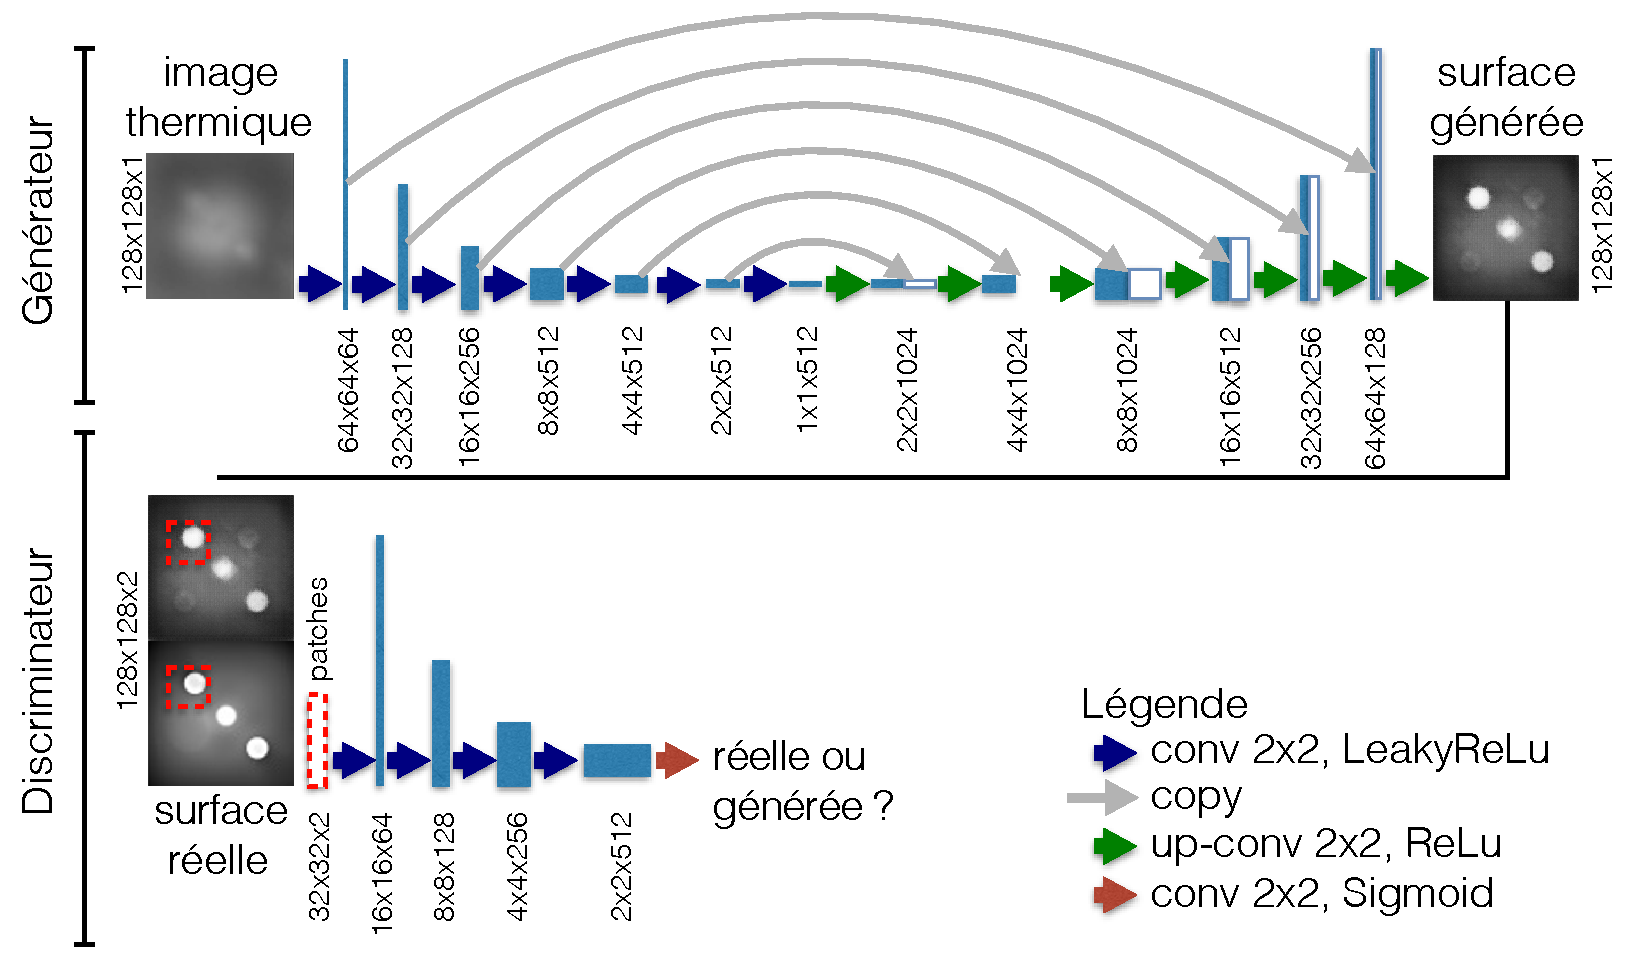
\includegraphics[width=\textwidth]{../Chap2/Figures/U-Net-architecture-JDD2018.pdf}
	\caption{Architecture du réseau antagoniste génératif \textit{U-Net}, utilisée par le modèle \textit{pix2pix}.}
	\label{fig:pix2pix}
\end{figure}

Nous avons évalué que l'utilisation de modèles polynomiaux ne permet pas de modéliser la relation entre une image thermique et une image géométrique.
Il est nécessaire de disposer d'un modèle qui est adapté au traitement d'images.
Les récentes avancées des réseaux de neurones profonds pour la transformation d'images nous ont poussé à évaluer l'utilisation de réseaux génératifs antagonistes (\textit{GAN}, détaillé dans le Chapitre \ref{ch:metric_learning} §\ref{subsubsec:GAN}).
% Les auto-encodeurs variationnels ne permettent pas de converger avec une telle précision avec un faible jeu de données. 
Nous avons utilisé la méthode \textit{pix2pix}, proposée par \citeauthor{zhu_unpaired_2017} \cite{zhu_unpaired_2017}.
La Figure \ref{fig:pix2pix} présente l'architecture du réseau de neurones \textit{U-Net}, qui est proposée par \citeauthor{ronneberger_unet_2015} \cite{ronneberger_unet_2015}.
Un réseau extrait l'information pertinente dans un vecteur de petites dimensions, appelé espace latent.
Le réseau génératif produit ensuite une image réaliste à partir de cette espace latent.
L'espace latent contient uniquement l'information pertinente pour reconstruire la géométrie de la pièce.

\begin{figure}[tbhp]
	\centering
	\begin{subfigure}[c]{0.48\textwidth}
		\includegraphics[width=\textwidth]{../Chap2/Figures/163-37_real_A.jpg}
		\caption{Image thermique de la pièce 10s après prod.}
	\end{subfigure}
	\begin{subfigure}[c]{0.48\textwidth}
		\includegraphics[width=\textwidth]{../Chap2/Figures/163-37_real_B.jpg}
		\caption{Image de l'altitude de la surface de la pièce.}
	\end{subfigure}
	\caption{Présentation d'un échantillon du jeu de données, en fausse couleur.}
	\label{fig:gan_dataset}
\end{figure}

Le jeu de données de notre étude est composé de couples d'images thermiques et d'images géométriques, présenté Figure \ref{fig:gan_dataset}
La valeur des pixels d'une image "géométrique" encode la mesure de hauteur de la surface.
La géométrie de la surface de la pièce est obtenue à l'aide d'un microscope confocal Altisurf 520\footnote{\href{https://www.altimet.fr/?page_id=236}{Spécifications techniques de l'Altisurf 520} sur le site Internet de la société Altimet.}.
Le réseau de neurones que nous utilisons est spécialisé dans le traitement d'images numériques de 8 bits.
Aussi, les images que nous utilisons sont normalisées sur 8 bits, soit sur une plage de valeurs entières de 0 à 255.
La perte de résolution de cette conversion est importante : le capteur thermique est précis à 0,05°C (ce qui ferait 2 000 valeurs entières), le microscope confocal à 0,1 micromètres (ce qui ferait 10 000 valeurs entières).
L'image thermique que nous utilisions a une résolution de 0,902°C, tandis que la carte d'élévation de la surface a une résolution de 1,57 micromètres.
% Une perspective à nos travaux sera d'utiliser un réseau de convolutions qui travaille avec des valeurs flottantes.
% La durée de l'apprentissage sera cependant nettement augmentée.

\begin{figure}[tbph]
	\centering
	\includegraphics[width=\textwidth]{../Chap2/Figures/sapristi_GAN_thermo_geo_testSet.pdf}
	\caption{Comparaison entre les images générées par le modèle à partir de l'image thermique et les images "géométriques" originales.}
	\label{fig:gan_results}
\end{figure}

La durée de l'apprentissage du modèle est de 3 heures pour 37 couples d'images.
Les poids de l'ensemble du réseau de neurones sont ajustés par apprentissage sur un jeu de données (méthode détaillée dans le Chapitre \ref{ch:metric_learning} §\ref{parag:neural_networks}).
Le jeu de données comporte 37 pièces.
Le nombre d'échantillons est faible car la durée de la mesure d'une pièce à l'aide du microscope confocal était de 45 minutes.
Une perspective directe est de réaliser cette étude sur un plus grand nombre d'échantillons et une variété de pièces.

Par la suite, nous évaluons la capacité du modèle appris à transformer une image thermique en image géométrique.
La Figure \ref{fig:gan_results} présente les résultats obtenus sur un jeu de données de test, qui n'a pas été utilisé pendant l'apprentissage.
Afin de mesurer la similarité entre les images originales et les images générées, nous calculons les indicateurs les plus utilisés dans la littérature de la compression d'images.
Nous n'avons pas réalisé de comparaison pixel à pixel car les images générées peuvent être légèrement translatées en comparaison des images originales.
Nous calculons les coefficients de Similarité Structurelle \textit{SSIM} proposée par \citeauthor{wang_image_2004} \cite{wang_image_2004} et le \textit{Peak Signal to Noise Ratio} pour la qualité de reproduction d'une image.
% La comparaison d'histogrammes est robuste aux transformations des images.
Enfin, nous utilisons la Décomposition Modale Discrète comme méthode de comparaison de la similarité entre deux images.
La Décomposition Modale Discrète décrit une image à partir de ses modes de vibrations spatiaux.
% C'est une méthode de décomposition qui produit un spectre représentatif de la géométrie, car les modes de vibrations sont ceux de plaques physiques.
Nous détaillons le principe de la Décomposition Modale Discrète dans la Section \ref{subsubsec:dmd}.
Le Tableau \ref{tab:gan_results} présente les résultats de ces comparaisons.

\begin{table}[tbhp]
	\centering
	\arrayrulecolor{black}
	\begin{tabular}{|l|c|c|}
		\arrayrulecolor{black}
		\hline
		Mesure de similarité & Moyenne & Écart-type \\
		\hline
		\hline
		Distance cosinus & 0,9 & 0,10 \\ \hline
		\hline
		Corrélation $R^2$ & 0,8 & 0,15 \\ \hline
		\textit{PSNR} & 18 & 3,95 \\ \hline
		\textit{SSIM} & 0,86 & 0,07 \\ \hline
		\hline
		\textit{Distance cosinus sur DMD} & 0,99 & 0,08 \\ \hline
		\textit{Corrélation $R^2$ sur DMD} & 0,98 & 0,04 \\ \hline
	\end{tabular}
	\caption{Performance du modèle pix2pix : similarité entre images générées et images originales.}
	\label{tab:gan_results}
\end{table}

La similarité moyenne sur les 14 pièces du jeu de données de test est élevée et l'écart-type global est faible.
Le jeu de données étant très petit, nous avons vérifié que la p-valeur est inférieure à 5\%, pour toutes les mesures de similarité.
La méthode \textit{pix2pix} permet d'extraire, de l'image thermique, de l'information sur la géométrie des pièces.


Bien que ces résultats soient encourageants, la durée de la phase d'apprentissage du modèle est de 3 heures sur une carte graphique puissante (\textit{Nvidia GTX 1080Ti}).
% Il n'est pour l'instant pas envisageable de construire ces modèles en ligne de production.
Il semble possible de pouvoir mettre à jour ce type de modèle à une fréquence journalière.
Enfin, la robustesse de ce modèle aux perturbations est également difficile à évaluer sur cette faible quantité de données et cet unique cas d'étude.
% Il sera néanmoins intéressant d'utiliser cette démarche lorsque de grandes quantités de données sur des cas d'études diverses seront disponible.

% TODO: Perspectives
% Une perspective intéressante est
% Dernièrement, \citeauthor{wu_learning_2016} montre que les réseaux génératifs antagonistes permettent de reconstruisent des représentations volumiques d'objet à partir d'une simple image \cite{wu_learning_2016}.
% La précision de la représentation de ces modèles est faible, car l' objectif est de représenter une grande diversité d'objets.
% Spécialiser ces modèles sur une unique pièce, pour augmenter la précision de la représentation volumique est aussi une perspective de recherche intéressante.

Dans notre recherche d'une méthode de contrôle des caractéristiques de la pièce, il reste à interpréter cette géométrie prédite.
Il s'agit  de comparer la géométrie obtenue à la géométrie cible, qui doit être celle du produit final.
Différentes méthodes de comparaison géométrique existent.
% Nous retiendrons l'apport du critère inertiel total, qui s'appuie sur le tolérancement inertiel généralisé aux formes tridimensionnelles par \citeauthor{adragna_proposition_2010} \cite{adragna_proposition_2010}.
% Si l'écart inertiel à la géométrique de référence de la pièce est grand, une alerte de non-qualité peut être déclenchée.
% Cependant, cette démarche nécessite de disposer de la géométrie cible sous un format informatisé.
% Cette information de référence est rarement disponible en injection-moulage ; en particulier car les outillages sont souvent retouchés au cours de leur vie, sans forcement numériser les retouches effectuées.
Cependant, nous souhaitons proposer une méthode de contrôle de la qualité des pièces la plus simplifiée possible.
C'est pourquoi nous choisissons pour la suite de notre travail de ne pas utiliser de modèle prédictif de la géométrie dans notre système de contrôle.
En revanche, nous utiliserons la démarche d'extraction de l'information à l'aide de réseau de neurones profonds, qui a ici montrée des possibilités intéressantes (voir le Chapitre \ref{ch:metric_learning}).

% Remarque : Dans le spectre infrarouge, l'état de surface des pièces plastiques ne permet pas la réflexion spéculaire.
% L'émission des pièces chaudes est isotrope.
% Cependant, la conductivité électrique de certains matériaux chargés en atome conducteur (carbone) supporte les propriétés spéculaires.
% Sur certaines pièces, en particulier celles pigmentées noires, des reflets de sources de chaleurs dans l'atelier de production parasitait l'imagerie thermique (moteurs de ponts roulants, chauffages ...).
% Il est possible de positionner un filtre polarisant devant la caméra thermique, orthogonal aux surfaces de la pièce, pour limiter ce problème.

\bigskip

\bigskip

\miniconclusion{Synthèse : thermographie pour le contrôle de la géométrie des pièces}{
	La conclusion principale de cette étude est que l'image thermique contient l'information de la géométrie
de la pièce finale.
	Ainsi, suivre une dérive de la géométrie revient à suivre une dérive de l'image thermique.

	Dans un objectif de contrôle de la qualité, l'analyse de l'image thermique permettrait de définir si une pièce est conforme ou est non-conforme, d'un point de vue géométrique.
}

\newpage
\section{Apport de la polarimétrie pour le contrôle des défauts d'aspect} \label{subsec:polarimetry}
La mesure du Degré de POlarisation Linéaire (DOLP) est utilisée dans de nombreux domaines techniques, dont le contrôle de la qualité de pièces composites\footnote{Le Fraunhofer Institute for Integrated Circuits IIS a présenté la \href{https://www.iis.fraunhofer.de/en/ff/sse/ims/tech/polarisationskamera.html}{solution de polarimétrie POLKA} pour le contrôle de pièces composites, lors du salon \href{https://www.control-messe.de/en/}{Control Stuttgart 2018}.} et de bouteilles en verre \cite{atkinson_highsensitivity_2018}.
Dans le cadre du moulage de polymères transparents, l'imagerie polarimétrique est couramment utilisée pour visualiser les contraintes mécaniques.
Les polymères transparents ont des propriétés de biréfringence qui sont induites par l'organisation interne des chaines des polymères \cite{denizart_thermal_1995}.
Les contraintes mécaniques appliquées à la pièce modifieront la biréfringence locale du matériau : c'est le phénomène optique de photoélasticité \cite{brewster_experiments_1833}.
Il est ainsi possible d'observer les contraintes mécaniques qui s'exercent.
Cependant, il n'existe pas à notre connaissance de travaux dans le domaine de la détection des défauts sur les pièces moulées en plastique.
C'est l'objet de l'étude présentée dans cette section.

\subsection{Polarimétrie pour mettre en valeur les défauts des pièces plastiques}
Les réflexions de la lumière à la surface d'un matériau peuvent être décomposées en une composante spéculaire et une composante diffuse \cite{hanrahan_reflection_1993}.
La composante lumineuse diffuse est causée par le phénomène de transluminescence (\textit{subsurface scattering}).
La lumière entre dans le matériau ; où elle est absorbée et dispersée ; avant de sortir du matériau.
% L'hypothèse lambertienne de la lumière diffuse n'est pas réaliste.
La lumière est alors absorbée et diffusée en fonction de sa longueur d'onde.
% De plus, le rayon lumineux est dispersé de nombreuses fois.
La lumière qui sort du matériau devient isotrope.  % et les direction de sortie des rayons sont aléatoire.

\begin{figure}[tbhp]
	\centering
	\includegraphics[width=\textwidth]{polarized_defect.pdf}
	\caption{Différentes composantes de réflexion d'un polymère semi-cristallin.}
	\textit{(a) réflexion spéculaire, (b) réflexion diffuse, (c) réflexion diffuse sur un défaut structurel du matériau, (d) réflexion spéculaire sur un défaut de forme géométrique. Figure inspirée de \cite{debevec_acquiring_2000}}.
	\label{fig:polarized_defect}.
\end{figure}

À partir de ces connaissances physiques, nous cherchons à utiliser la mesure de l'angle de polarisation pour la détection de défauts sur les pièces plastiques.
La Figure \ref{fig:polarized_defect} présente l'effet de différents défauts sur la polarisation de la lumière réfléchie.
La réflexion spéculaire est représentée par le rayon (a).
La réflexion diffuse est représentée par le rayon (b).

Dans le cadre des matériaux semi-cristallins, nous posons deux hypothèses importantes pour la polarisation des réflexions :
\begin{itemize}
	\item Un défaut géométrique (forme, retassure, rayure)  modifie la courbure de la surface, ainsi il modifie l'angle de polarisation de la réflexion spéculaire : réflexion (d) Fig. \ref{fig:polarized_defect}.
	\item Un défaut qui modifie la structure de la matière (brûlure, givrage, pollution) diffuse la lumière incidente, ainsi la lumière que le défaut réfléchit est diffuse ; elle ne possède pas de composante spéculaire : réflexion (c) Fig. \ref{fig:polarized_defect}.
\end{itemize}
% Il n'existe pas, à notre connaissance, d'étude qui concernent l'utilisation de la polarimétrie pour le contrôle des défauts sur des pièces plastiques.
Dans la suite de cette section, nous évaluerons l'intérêt de la polarimétrie pour la mise en valeur des défauts sur un cas d'application industriel.
% De précédents travaux proposent d'utiliser la polarimétrie pour la segmentation des objets.
% Intérêt de la polarimétrie : mise en valeur des défauts géométrique.
Si nos hypothèses sont vérifiées, cela permettra de mettre en valeur séparément les défauts géométriques à l'aide de la composante spéculaire et les défauts de la structure de la matière à l'aide de la composante diffuse.
Pour des questions de coût de l'équipement, nous utiliserons un capteur polarimétrique que nous avons conçu.

% La modélisation des phénomènes lumineux est un enjeu important des rendus graphiques photo-réalistes.
% Jusqu'en 1993, la composante diffuse est considérée comme lambertienne (orthotrope).
% \citeauthor{hanrahan_reflection_1993} \cite{hanrahan_reflection_1993} propose de modéliser la réflection diffuse à partir des propriétés de réflections des différentes couches successives qui composent un matériau et qui ont des propériétés optiques différentes.

La mesure des composantes de réflexions spéculaires et diffuses d'un matériau est un enjeu important pour les rendus d'images photo-réalistes.
En 1997, \citeauthor{nayar_separation_1997} \cite{nayar_separation_1997} propose de mesurer la composante spéculaire, séparément de la composante diffuse, en utilisant un filtre polarisant.
Selon les équations de Fresnel, une réflexion spéculaire est linéairement polarisée selon son plan d'incidence : réflexion (a) Fig. \ref{fig:polarized_defect}.
À contrario, une réflexion diffuse n'est pas polarisée : réflexion (b) Fig. \ref{fig:polarized_defect}.

%\begin{figure}[htpb]
%	\centering
%	\begin{subfigure}[c]{0.33\textwidth}
%		\centering
%		\includegraphics[width=\textwidth]{imgOriginal.pdf}
%		\caption{Image originale}
%	\end{subfigure}
%	\begin{subfigure}[c]{0.33\textwidth}
%		\centering
%		\includegraphics[width=\textwidth]{imgDiffuse.pdf}
%		\caption{Composante diffuse}
%	\end{subfigure}
%	\begin{subfigure}[c]{0.33\textwidth}
%		\centering
%		\includegraphics[width=\textwidth]{imgSpecular.pdf}
%		\caption{Composante spéculaire}
%	\end{subfigure}
%	\caption{Acquisition des composantes de réflexions spéculaire et diffuse.}
%	\label{fig:specular_diffuse}
%\end{figure}

\begin{figure}[bhtp]
	\begin{center}
		\begin{tabular}{c}
			\includegraphics[width=\textwidth]{imgComponentsR.pdf}
			\\
			(a) Image originale \hspace{1.4cm} (b) Composante diffuse \hspace{1.4cm} (c) Composante spéculaire
		\end{tabular}
	\end{center}
	\caption{Acquisition des composantes de réflexions spéculaire et diffuse.}
	\label{fig:specular_diffuse}
\end{figure}
En positionnant un filtre polarisant linéaire devant une caméra et en l'orientant selon un angle orthogonal à l'angle d'incidence de la source lumineuse, on capture uniquement la composante diffuse \cite{debevec_acquiring_2000}.
La même démarche, réalisée avec le polarisant orienté selon le même angle que l'angle d'incidence, permet de capturer la composante spéculaire, ainsi que la moitié de la composante diffuse.
Il est alors possible de séparer la réflexion spéculaire et la réflexion diffuse, telle que la Figure \ref{fig:specular_diffuse} le montre.
Sur ces images, on observe que, selon l'hypothèse émise, les défauts de forme géométrique du fond de la boîte sont mis en valeur dans l'image spéculaire, mais pas dans l'image diffuse.
En revanche, les défauts qui ont modifiés la structure de la matière (ici des tâches de givrage et des impuretés) apparaissent peu dans l'image spéculaire, mais ils sont présents, de couleur sombre, dans l'image diffuse.
Dans la suite de ce travail, nous chercherons à évaluer quantitativement l'apport de la polarimétrie pour les performances de la détection des défauts.

\subsection{Conception d'un capteur polarimétrique bas-coût}
Les capteurs polarimétriques commerciaux actuellement disponibles sont coûteux (> 5000€).
Cela s'explique par les technologies complexes qu'ils emploient pour obtenir une résolution élevée de la mesure du Degré de Polarisation Linéaire (DoLP).
Cela nécessite un processus de calibration long.
Aussi, ces capteurs sont principalement utilisés à des fins de recherches ou d'applications de surveillance civile et militaire.

Différentes méthodes de conception d'un capteur polarimétrique existent \cite{tyo_review_2006}.
La méthode la plus classique utilise 3 ou 4 caméras, qui imagent chacune la lumière selon un angle de polarisation linéaire différent.
Plusieurs caméras sont superposées et un chemin optique spécialement conçu aligne précisément l'image des différentes caméras pour compenser la différence de parallaxe.
Les miroirs sans-teints sont couramment utilisés pour supprimer la parallaxe entre deux caméras \cite{wolff_polarization_1995}.
Dans le cas où 3 caméras, ou plus sont utilisées, des miroirs et des prismes deviennent nécessaires.
C'est le principe de la \textit{division d'amplitude}.

La méthode de la \textit{division du temps} utilise une caméra haute vitesse et un filtre polarisant, en rotation synchronisée avec la fréquence d'acquisition du capteur.
Cela limite le nombre d'images par secondes de l'acquisition et cela limite la durée de vie à cause du système rotatif.
Dans la même démarche, le filtre polarisant peut être remplacé par des cristaux liquides \cite{gendre_full_2011}.
% Cancellation of motion artifacts caused by a division-of-time polarimeter, Marconnet, Gendre, Foulonneau, Bigué (2011)

Les capteurs polarimétriques peuvent aussi être construits avec un capteur unique.
On parle de \textit{division de l'ouverture} lorsque la surface du capteur est séparée pour acquérir différents degrés de polarisation.
Plusieurs lentilles focalisent une image, qui a été polarisée par un filtre, sur une région différente du capteur.
Cette méthode nécessite une compensation de l'écart de parallaxe créé par l'écart des différentes lentilles \cite{riou_calibration_2015}.  % riou=550x550

\begin{figure}[bht]
	\centering
	\includegraphics[width=0.85\textwidth]{Polarimetric_imager_overview_and_calibration.jpg}
	\caption{Notre polarimètre et le procédé de calibration par homographie.}
	\label{fig:sensor}
\end{figure}

Enfin, on parle de \textit{division du plan focal} lorsque ce sont les pixels du capteur qui sont directement polarisé.
Des filtres polarisés sont directement intégrés sur le plan du capteur \cite{yamazaki_fourdirectional_2016} (CMOS Sony \textit{IMX250-MZR}, 5 millions de pixels\footnote{\href{https://www.sony-semicon.co.jp/products_en/IS/sensor5/index.html}{Informations sur le capteur polarimétrique \textit{IMX250-MZR}}, sur le site Internet du fabriquant Sony.}).
Cela supprime la complexité optique, mais réduit la résolution finale de l'image par un facteur 4.
Il est possible d'interpoler entre les angles de polarisation pour limiter cette perte, à la manière de la reconstruction d'une image couleur à partir de la matrice de filtre de Bayer.
Le capteur \textit{IMX250-MZR} dispose néanmoins d'une résolution d'acquisition de $2448\times 2048$ pixels, soit une résolution  de $1223\times 1023$ pixels, ce qui est suffisant pour utiliser nos algorithmes.

Nous avons étudié la possibilité de réalisation d'un capteur polarimétrique au coût limité (inférieur à 1000€), avec une résolution satisfaisante de $1920\times 1080$ pixels \cite{nagorny_polarimetric_2019}.
En comparaison, le coût des caméras basées sur un capteur à division de plan focal est de l'ordre de 2000€.

Nous avons choisi de ne pas utiliser de système optique pour simplifier la construction.
Notre capteur repose sur la fusion de trois caméras polarisées par des filtres linéaires à 0°, 60° et 120° (voir la Figure \ref{fig:sensor} (a)).
Ces trois angles, espacés de 60°, permettent de modéliser l'ensemble du disque de polarisation linéaire dans la sphère de Poincaré\footnote{Pour reproduire la sphère de Poincaré, il est nécessaire de mesurer également la composante de polarisation circulaire, ce que nous ne faisons pas ici}.
Une source de lumière polarisée linéairement à 0° éclaire les pièces.


\subsubsection{Choix des capteurs et correction de parallaxe}
Nous utilisons des webcams grands publics Logitech C922\footnote{\href{https://www.logitech.fr/fr-fr/product/c922-pro-stream-webcam}{Informations sur la webcam C922} sur le site Internet de la société Logitech.}, pour leurs simplicités d'implémentation en USB et leurs qualités en condition de basse luminosité.
Des caméras industrielles plus robustes peuvent être utilisées avec la même méthode.

Afin de compenser la parallaxe, sans système optique, nous utilisons une transformation logicielle.
Dans un premier temps, nous calibrons la position du plan de fusion à l'aide d'une planche de référence composée de marqueurs \textit{ChAruco} \cite{garrido-jurado_automatic_2014, garrido-jurado_generation_2016, romero-ramirez_speeded_2018}.
Ensuite, nous utilisons la bibliothèque \textit{OpenCV} \cite{opencv_library} pour calculer une transformation homographique entre les trois caméras (voir la Figure \ref{fig:sensor} (c)).
La détection des marqueurs et l'association entre deux images est présentée dans la Figure \ref{fig:mecaruco}.
Le logiciel de fusion polarimétrique est distribué sous licence libre MIT, sous la forme d'un paquet Python.
Le code source du paquet \href{https://github.com/a1rb4Ck/camera-fusion}{camera-fusion est disponible en ligne}.

\begin{figure}[thb]
	\centering
	\includegraphics[width=\textwidth]{vis_matches.jpeg}
	\caption{Détection et association de marqueurs \textit{ChAruco} entre deux caméras.}
	\label{fig:mecaruco}
\end{figure}

Il est important de noter que la parallaxe est compensée sur un plan unique.
Ainsi, le vecteur de Stokes ne peut être reconstruit que dans ce plan.
La parallaxe est une limite importante de notre système lorsque la surface de l'objet que l'on mesure n'est pas située sur le plan de la calibration.
La différence de parallaxe dans notre système pourrait être exploitée.
Une perspective intéressante à nos travaux serait d'utiliser la théorie \textit{light-field}, à partir des 3 caméras qui possèdent un point de vue différent \cite{wilburn_high_2005}.
Il serait alors possible d'obtenir une information de polarimétrie en fonction de la distance, tel que le travail de \citeauthor{gendre_interest_2018} \cite{gendre_interest_2018} le propose.
La reconstruction d'une carte de profondeur de la scène est également possible.
La précision attendue n'est pas de l'ordre du micromètre, mais cette information complémentaire pourrait être utile afin d'évaluer la géométrie globale d'une pièce.

Cependant, afin de ne pas avoir à réaliser de calibration, notre approche est de ne pas corriger la parallaxe pour l'analyse des images. 
Nous analyserons les données brutes issues des capteurs, afin de classifier la qualité des pièces.

\subsubsection{Dimensionnement de la source lumineuse polarisée}
La Figure \ref{fig:raw_measures} présente les images brutes pour une unique pièce.
Dans ce cas spécifique, on observe que la dernière image est plus sombre que les autres.
Cela est dû au fait que l'angle du filtre polarisant linéaire situé devant la caméra est orthogonale à l'angle de polarisation linéaire de la source lumineuse.
La Figure \ref{fig:specular_diffuse} utilise cette propriété pour séparer les réflexions diffuses et les réflexions spéculaires.
% Cela peut être limitant pour le bruit de cette image, dans le cas où la sensibilité du capteur est trop limitée.
% Donc il est recommandé de ne pas orienter les filtres des caméras perpendiculaires à la polarisation de la source lumière.

\begin{figure}[htbp]
	\centering
	\includegraphics[width=\textwidth]{stats_part151-1.png}
	\caption{Images de la même pièce par les 3 caméras, sous 3 angles de polarisation différents.}
	\label{fig:raw_measures}
\end{figure}

Enfin, nous avons évalué qualitativement dans des ateliers de production l'effet de la lumière ambiante, non polarisée, sur la qualité de nos mesures.
Nous employons une source lumineuse puissante de 8000 lumens pour pouvoir négliger l'effet de la lumière ambiante.
Nous estimons que la moitié de la luminosité est perdue par la polarisation.
Grâce au dimensionnement de notre source lumineuse, nous n'avons pas observé de problème lors des essais en atelier.
En effet, les zones situés à proximité direct des machines sont souvent peu éclairées, car l'éclairage des ateliers est traditionnellement au plafond ; il est éloigné de plusieurs mètres des machines, tandis que notre dispositif mesure des pièces à une distance maximale d'un mètre.
Nous recommandons néanmoins de vérifier qu'aucune source lumineuse directe ne risque de polluer les mesures.
Une perspective à nos travaux sera d'évaluer quantitativement l'effet de la lumière ambiante non polarisée sur les performances de notre système.

\subsubsection{Reconstruction du vecteur partiel de Stokes}
L'équation de \citeauthor{stokes_composition_1851} \ref{eq:stokes_equation} permet de connaitre l'intensité lumineuse de la réflexion, pour un degré de polarisation $\theta$ \cite{stokes_composition_1851} :
\begin{equation} \label{eq:stokes_equation}
	I(\theta,\Phi) = \frac{1}{2}[S_0+S_1\cos 2\theta+S_2\cos \Phi \sin 2\theta+S_2\sin \Phi \sin 2\theta]
\end{equation}

À l'aide de notre dispositif, nous mesurons l'intensité lumineuse pour trois angles de polarisation linéaires $\theta$ espacés de 60° ; mais nous ne mesurons pas l'angle de polarisation circulaire $\Phi$ que nous définissons arbitrairement à zéro.
Nous supposons que nos filtres polarisants sont idéaux et polarisent complètement la lumière.
Aussi, nous négligeons la transmittance perpendiculaire à leur angle de polarisation effective.
À partir de \ref{eq:stokes_equation}, nous obtenons les Équations \ref{eq:IO}, \ref{eq:I60}, \ref{eq:I120} :

\begin{equation} \label{eq:IO}
	I(\theta=0\degree) = \frac{1}{2}\left[S_0 + S_1\right]
\end{equation}
\begin{equation} \label{eq:I60}
	I(\theta=60\degree) = -\frac{1}{4} S_0 + \frac{1}{2} \sqrt{\frac{3}{2}} S_2
\end{equation}
\begin{equation} \label{eq:I120}
	I(\theta=120\degree) = -\frac{1}{4} S_0 - \frac{1}{2} \sqrt{\frac{3}{2}} S_2
\end{equation}

On obtient le vecteur partiel de \citeauthor{stokes_composition_1851} de la lumière réfléchie \ref{eq:stokeVector} \cite{li_method_2014} :

\begin{equation}
	S_{partiel} =
	\left(\!\!\!
		\begin{array}{c}
			S_0 \\
			S_1 \\
			S_2
		\end{array}
	\!\!\!\right) =
	\left(\!\!\!
		\begin{array}{c}
			I \\
			Q \\
			U
		\end{array}
	\!\!\!\right) =
	\left(\!\!\!
		\begin{array}{c}
			\frac{1}{3} I_{0} + \frac{1}{3} I_{60} + \frac{1}{3} I_{120} \\
			\frac{2}{3} I_{0} - \frac{1}{3} I_{60} -  \frac{1}{3} I_{120} \\
			\frac{1}{2 \sqrt{\frac{3}{2}}} \ I_{60} - \frac{1}{2 \sqrt{\frac{3}{2}}} I_{120}
		\end{array}
	\!\!\!\right)
	\label{eq:stokeVector}
\end{equation}
% I0                |   sqrt(3/2) I0  +   sqrt(3/2) I60  +   sqrt(3/2) I120 |   I0
% Q0 = 1/3sqrt(3/2) | 2*sqrt(3/2) I0  +  -sqrt(3/2) I60  +  -sqrt(3/2) I120 |  I60
% U0                |           0 I0  +         1,5 I60  +        -1,5 I120 | I120

\begin{figure}[tbph]
	\centering
	\begin{subfigure}[l]{0.495\textwidth}
		\includegraphics[width=\textwidth]{../Chap2/Figures/imgOriginal.pdf}
		% \caption{Image originale}
	\end{subfigure}
	\begin{subfigure}[r]{0.495\textwidth}
		\includegraphics[width=\textwidth]{../Chap2/Figures/img_stokesI.pdf}
		% \caption{Paramètre de Stokes S_0 : I}
	\end{subfigure}
	\vspace{1cm}
	\\
	\begin{subfigure}[l]{0.495\textwidth}
		\includegraphics[width=\textwidth]{../Chap2/Figures/img_stokesQ.pdf}
		% \caption{Paramètre de Stokes S_1 : Q}
	\end{subfigure}
	\begin{subfigure}[r]{0.495\textwidth}
		\includegraphics[width=\textwidth]{../Chap2/Figures/img_stokesU.pdf}
		% \caption{Paramètre de Stokes S_2 : U}
	\end{subfigure}
	\vspace{1cm}
	\\
	\begin{subfigure}[l]{0.495\textwidth}
		\includegraphics[width=\textwidth]{../Chap2/Figures/img_polDoLP.pdf}
		% \caption{Degré de Polarisation Linéaire DoLP}
	\end{subfigure}
	\begin{subfigure}[r]{0.495\textwidth}
		\includegraphics[width=\textwidth]{../Chap2/Figures/img_polAoP.pdf}
		% \caption{Angle de Polarisation Linéaire AoP}
	\end{subfigure}
	\caption{Reconstruction des paramètres de Stokes partiels, du Degré et de l'Angle de Polarisation, à partir des images de 3 caméras.}
	\label{fig:stokes_reconstruction}
\end{figure}

La Figure \ref{fig:stokes_reconstruction} présente les résultats de reconstruction obtenus.
On observe les erreurs dues à la parallaxe sur une pièce qui n'est ici pas plane.
Les mesures sur le fond de la boîte sont néanmoins exploitables.
Cette évaluation est actuellement qualitative.
Une perspective de ce travail sera d'évaluer la justesse de notre reconstruction sur des échantillons optiques de références.


\subsection{Apport de la polarimétrie sur les performances d'un classifieur de la qualité}
% \subsubsection{Exploitation des données}
\label{subsubsec:pola_results}

Dans \citetitle{nagorny_polarimetric_2019}, nous évaluons l'apport de la polarimétrie pour la détection des défauts sur les pièces plastiques \cite{nagorny_polarimetric_2019}.
Nous réalisons notre étude sur le jeu de donnée de 204 pièces "boîte noires", qui est présenté dans le Chapitre \ref{ch:dataset} §\ref{subsec:l12_doe}.
Les paramètres de la machine ont été variés suivant un plan d'expériences de criblage ; aussi, le jeu de donnée est composé de pièces qui possèdent une variété de défauts.
La qualité de chaque pièce a été évaluée selon la méthode présentée dans le Chapitre \ref{ch:dataset} §\ref{parag:offline_annotation}.
À partir de cette évaluation, nous définissons deux types de pièces sur notre échelle de qualité : les pièces conformes dont l'indice de qualité est inférieur à 3, et les pièces non-conformes dont l'indice est supérieur.
Les images enregistrées ont une résolution de $1920 \times 1200$ et nous avons dû sous-échantillonner cette résolution à $331 \times 331$ pixels pour réaliser l'analyse sur notre infrastructure informatique.

Nous comparons les performances d'algorithmes de classification de la qualité dans trois cas :
\begin{itemize}
	\item 
	Sans éclairage polarisé, ni filtres polarisants sur les caméras (\textit{dataset\_bench}),
	\item 
	sans éclairage polarisé, mais avec des filtres polarisés sur les caméras (\textit{dataset\_nopola}),
	\item avec éclairage polarisé et filtres polarisés sur les caméras (\textit{dataset\_pola}).
\end{itemize}
La Figure \ref{fig:raw_measures} présente les images obtenues dans les trois cas par notre système.
La classification est réalisée sur les images brutes issues des capteurs.
Nous n'avons pas compensé la parallaxe, ni pré-traité les images.
Nous discutons de l'intérêt du pré-traitement d'images dans la section suivante §\ref{subsec:image_preprocessing}.

Dans le cadre de cette étude, l'algorithme d'apprentissage est considéré comme le meilleur possible, afin de négliger son influence.
L'algorithme d'apprentissage est choisi et il est optimisé automatiquement par la méthode \textit{TPOT}, qui est détaillée dans le Chapitre \ref{ch:metric_learning} §\ref{subsec:evolution}.
La durée de l'apprentissage du meilleur classifieur est de 15 heures.

\begin{table}[hbtp]
	\begin{center} 
		\begin{tabular}{|c|c|c|c|}
			\hline
			Angle & \textit{dataset\_pola} & \textit{dataset\_nopola} & \textit{dataset\_bench}\\
			\hline
			\hline
			3 angles   & \textbf{0,921} & 0,851 & \textbf{0,948} \\
			0\degree   &         0,841  & 0,831 & \textbf{0,923} \\
			60\degree  &         0,853  & 0,851 &         0,820  \\
			120\degree &         0,812  & 0,830 & \textbf{0,889} \\
			\hline
		\end{tabular}
	\end{center}
	\caption{Comparaison des scores de justesse de classification de la non-conformité.}
	\label{tab:perfAutoML}
\end{table}

Le Tableau \ref{tab:perfAutoML} présente les scores de justesse obtenus avec le meilleur algorithme de classification, pour différentes conditions d'éclairage et de polarisation.
La première ligne indique le score dans le cas où les images des trois caméras ont été utilisées.
Les images brutes des capteurs sont concaténées dans une matrice de dimensions $993\times 331$.
Les lignes suivantes indiquent le score dans le cas où seule une caméra polarisée à un certain angle est utilisée.
La première colonne est le score obtenu avec un éclairage polarisé.
La seconde colonne est le score obtenu avec un éclairage non polarisé.
Enfin, la dernière colonne est une mesure de référence : aucune caméra n'est polarisée et l'éclairage n'est pas polarisé.

On observe que l'utilisation des 3 caméras polarisées et de l'éclairage polarisée permet d'obtenir un score de classification plus élevé (justesse de 0,921).
La polarimétrie semble apporter de l'information pour améliorer la détection des pièces conformes.

En revanche, l'utilisation des 3 caméras sans polarisation permet d'obtenir un score plus élevé que le système polarisé.
Nous expliquons ce résultat par le fait qu'il existe de l'information supplémentaire pertinente dans la fusion des trois points de vue.
De plus, les filtres polarisants pourraient dégrader une partie de cette information issue des trois caméras.
Enfin, il est possible que notre système à faible coût occasionne un biais pour les données.
Nous n'avons pas réussi à mettre en évidence de biais.
Une perspective importante de nos travaux sera de réaliser la même étude à l'aide d'un polarimètre calibré, afin de valider définitivement si c'est la polarimétrie qui apporte de l'information, ou bien les différents points de vue des caméras.

\bigskip

\bigskip

\miniconclusion{Synthèse : polarimétrie pour le contrôle des défauts d'aspect}{
	Notre étude montre l'intérêt de la polarimétrie pour la mise en valeur des défauts sur les pièces plastiques.

	Les variations de la courbure de la géométrie des pièces peuvent être observées par la variation de l'angle de polarisation des réflexions spéculaires.
	Cela permet de mettre en évidence les défauts de retassure.
	
	Les défauts qui modifient la structure de la matière peuvent être observés dans les réflexions diffuses, qui ne sont pas polarisées. 

	Pour le contrôle de la qualité, l'analyse de l'imagerie polarimétrique permettrait de déterminer le type de défaut en présence.
	Une étude approfondie reste à réaliser pour valider quantitativement l'intérêt de la polarimétrie, en comparaison de la seule analyse de plusieurs points de vue.
}
\newpage

\section{Traitement et fusion de l'information issue de mesures multimodales} \label{sec:multimodal}
Dans le cadre de nos travaux, nous avons évalué l'intérêt de deux techniques d'imageries non-conventionnelles, polarimétrie et thermographie, pour la mesure des caractéristiques d'une pièce.
Nous cherchons désormais à combiner ces mesures.
De nombreuses méthodes de fusions multimodales peuvent être appliquées.

Dans notre étude sur l'apport de la polarimétrie §\ref{subsubsec:pola_results} \cite{nagorny_polarimetric_2019}, nous proposons de concaténer les images issues des capteurs et d'exploiter cette donnée en utilisant l'apprentissage statistique.
Cette démarche peut être réalisée en ajoutant une image thermique aux données.
On parle de "fusion amont" des données.
Cette démarche est intéressante car un algorithme d'apprentissage statistique va pouvoir apprendre de la relation entre les différentes mesures.
C'est la démarche que nous choisissons d'employer dans nos travaux.

Sur ces données concaténées, il est possible d'appliquer un méthode de réduction de l'information §\ref{subsec:statistical_descriptor}.
Il est important que cette méthode ne détruise pas l'information pertinente contenue dans les mesures.
C'est pourquoi nous avons privilégié dans nos travaux les méthodes de réduction de l'information par apprentissage non-supervisé.
Dans le Chapitre §\ref{ch:metric_learning}, nous comparons différentes méthodes d'apprentissage non-supervisées sur nos données.

Dans cette section, nous présenterons en particulier les méthodes de filtrages que nous avons évaluées sur nos données.
% Synthetic Sensor \citeauthor{laput_synthetic_2017} \cite{laput_synthetic_2017}.
Enfin, nous détaillerons l'intégration logicielle des méthodes de fusion sur système embarqué, dans le Chapitre \ref{ch:theeye}.

\subsection{Nécessité de l'extraction de l'information pertinente} \label{subsec:extraction}
Nous supposons dans cette section que l'information pertinente est contenue dans les mesures issues des capteurs.
Aucun algorithme ne peut extraire de l'information si elle n'existe pas.
% Nous avons discuté de la pertinence des mesures thermique et polarimétrique dans la Section\ref{sec:non_conventional_imaging}.
% La performance d'un dispositif de mesure est lié à l'association de moyens de mesure pertinent et d'algorithmes de traitement adaptés.

Une perspective de nos travaux est de proposer l'ajustement en boucle fermée de la qualité des pièces.
C'est pourquoi notre système de contrôle de la qualité doit respecter le temps de cycle du procédé, afin de pouvoir corriger les paramètres du procédé dès la pièce suivante.
Doivent être inscrits dans le temps de cycle de production d'une pièce : le déplacement de la pièce devant le système de mesure, la durée de la mesure et la durée de l'analyse de la mesure.
Si la durée de la mesure est de 10 secondes, la durée de l'analyse des mesures doit être proche de la seconde.
Le contexte industriel demande une grande fiabilité  et le respect de cette durée d'analyse de la mesure.

Nous avons évalué la faisabilité industrielle d'un traitement des mesures sur serveur distant (\textit{Cloud}), qui disposent de moyens de calcul performants.
La durée des calculs sur ces serveurs est de l'ordre de la milliseconde.
En pratique, ce sont les problèmes de latence des réseaux informatiques qui ne permettent pas d'être certain d'une réponse inférieure à la seconde.
% En effet, nous avions envisagé de réaliser l'inférence sur un serveur distant, cependant la majorité des ateliers n'est pas équipée en infrastructure de réseau informatique filaire au pied des machines.
% En pratique, nous avons eu des problèmes insolubles de latence sur les infrastructures réseaux radiofréquence présentes dans certains ateliers de production.
% en émission sur la connexion radio-fréquence (WiFi) qui ne permettait pas de réaliser l'inférence à distance.
% Les données mesurées peuvent atteindre un méga octet par pièce et les pertes de paquets sur la connexion WiFi sont dues au mouvement des bras robotiques préhenseurs métalliques.
Sans évolution de l'infrastructure réseau dans les ateliers de production, au vue de cette contrainte temporelle, la réalisation de l'analyse des mesures doit être effectuée sur un système de calcul embarqué, au plus proche des moyens de mesure.

Aussi, plus la dimension de l'information issue des capteurs est réduite, plus l'inférence est rapide.
% L'inférence de modèles d'apprentissage supervisé, dont les réseaux de neurones profonds, est inférieur à la seconde.
La réduction de dimensions est aussi appelée "extraction de l'information" ou "compression de l'information".

% Enfin, la réduction de l'information est un objectif crucial afin de pouvoir piloter en boucle fermée le procédé.
% En effet, le pilotage multivarié des procédés industriels est possible dans un espace de dimensions faibles (de dimensions dix à cent).

Dans cette section, nous discutons de l'intérêt du traitement des images obtenues par nos capteurs, en amont de l'analyse des mesures §\ref{subsec:image_preprocessing}.
Puis nous présentons notre méthode d'extraction de l'information pertinente, à l'aide d'une sélection automatique de descripteurs statistiques §\ref{subsec:features_selection}.

\subsection{Traitement d'images amont} \label{subsec:image_preprocessing}
Nous avons étudié la possibilité de mettre en valeur la présence des défauts d'aspect que nous souhaitons détecter.
Notre hypothèse est simple : si un traitement d'image fait ressortir les défauts pour la vision d'un humain, ce traitement améliorera les performances du système informatique de détection des défauts.

Nous avons étudié l'effet de différentes méthodes de traitement d'image sur la performance de la classification de la qualité des pièces.
La Figure \ref{fig:preprocessing} présente les différents traitements étudiés.

\begin{figure}[tbhp]
	\begin{center}
		\begin{tabular}{c}
			\begin{subfigure}[b]{0.245\linewidth}
				\includegraphics[width=3.7cm]{img_r.jpg}
				\caption{$0$\degree, $45$\degree, $90$\degree$\rightarrow$RGB}
			\end{subfigure}
			\begin{subfigure}[b]{0.245\linewidth}
				\includegraphics[width=3.7cm]{img_sub_r.jpg}
				\caption{Différence à $0$\degree$\rightarrow$RGB}
			\end{subfigure}
			\begin{subfigure}[b]{0.245\linewidth}
				\includegraphics[width=3.7cm]{img_gauss7x7_sobel_r.jpg}
				\caption{Diff.+gaussien+Sobel}
			\end{subfigure}
			\begin{subfigure}[b]{0.245\linewidth}
				\includegraphics[width=3.7cm]{img_gauss7x7_sobel_hist_r.jpg}
				\caption{(c) avec histo. optimisé}
			\end{subfigure}
		\end{tabular}
	\end{center}
	\caption{Illustration de différentes méthodes de pré-traitements des images issues des trois caméras polarisées.}
	\label{fig:preprocessing}
\end{figure}

En pratique, nous n'avons pas réussi à valider notre hypothèse.
Toutes les méthodes de traitement que nous avons implémentées ont diminuées les performances de classification.
Le traitement d'image semble détruire une partie de l'information pertinente.
Aussi, à défaut de trouver un traitement idéal, nous recommandons de ne pas réaliser de traitement d'images et d'analyser les données brutes issues des capteurs.
C'est l'intérêt des méthodes d'apprentissage statistique pour exploiter les données brutes.
Ils construisent la méthode de traitement la plus appropriée de manière automatique.

\subsection{Descripteurs statistiques} \label{subsec:statistical_descriptor}
Nous utilisons des descripteurs de référence de la littérature.
À contrario des méthodes présentées dans le Chapitre \ref{ch:metric_learning}, il n'y a pas d'apprentissage.
C'est l'humain qui conçoit les fonctions mathématiques des descripteurs.
La limite à cette démarche est le manque de variété des descripteurs disponibles.
À contrario, les méthodes par apprentissage de réseau de neurones permettent de créer des descripteurs spécifiquement adaptés aux problèmes à résoudre.
Le réseau de neurones va apprendre la méthode : c'est la démarche de l'apprentissage de bout-en-bout (\textit{end to end learning}) : à partir des données brutes ont obtient le résultat attendu.

Dans notre étude \citetitle{nagorny_quality_2017}, nous avons choisi de balayer un large spectre de la vision par ordinateur \cite{nagorny_quality_2017}.
25 descripteurs statistiques ont été évalués :
\begin{itemize}
	\item statistiques d'ordre inférieur à 2 :
		\subitem minimum,
		\subitem maximum,
		\subitem moyenne,
		\subitem médiane,
		\subitem mode,
		\subitem écart-type,
		\subitem quantile 75 et 90,
	\item statistiques d'ordre supérieur :
		\subitem quantile 75\% et 90\%,
		\subitem assymétrie (\textit{skewness}),
		\subitem coefficient d’aplatissement (\textit{kurtosis}),
		\subitem 14 paramètres de \citeauthor{haralick_textural_1973},
		\subitem 100 premiers modes de la Décomposition Modale Discrète.
\end{itemize}

Nous détaillerons le principe des paramètres de Haralick §\ref{subsubsec:haralick} et de la Décomposition Modale Discrète §\ref{subsubsec:dmd} dans les paragraphes suivants.
% - Décomposition Modale Discrète, utilisée avec succès dans les travaux de doctorat de Thomas Lacombe \cite{lacombe_exploitation_2018a}.

\subsubsection{Description de la texture d'une image : paramètres de Haralick} \label{subsubsec:haralick}
En 1973, \citeauthor{haralick_textural_1973} proposent 14 paramètres pour décrire la texture d'une image \cite{haralick_textural_1973}.
Les travaux de doctorat de \citeauthor{lacombe_exploitation_2018a} utilisent avec succès les paramètres de Haralick pour décrire des images, dans un objectif  d'automatisation du contrôle de la qualité de pièces plastiques.
Les paramètres de Haralick ont été largement utilisés dans la littérature du traitement d'images.
C'est pourquoi nous avons étudié leurs apports pour la description de nos images thermiques et polarimétriques.

La méthode de Haralick nécessite le calcul de la matrice des co-occurrences des pixels voisins de l'image, appelée \textit{Gray-Level Co-occurrence Matrix}.
La matrice de co-occurrence $G$ est carrée, de dimension $N_g$ le nombre de niveau de luminance dans l'image.
Pour une image classique 8 bits, $N_g = 256$.
La matrice $G$ est constituée de couples de valeur $P_{i, j}$ qui indiquent le nombre d'occurrence où un pixel de valeur $i$ est adjacent à un pixel de valeur $i$, Équation \ref{eq:cooccurrence}.
Pour une image 8 bits, on aura $255^2$ couples $p$.
\citeauthor{haralick_textural_1973} proposent d'évaluer les co-occurrences entre les pixels selon 4 directions $\theta = 0, \ \frac{\pi}{2}, \ \frac{3\pi}{4}, \ \pi$.

\begin{equation} \label{eq:cooccurrence}
\mathbf{G}=\left[\begin{array}{cccc}{p(1,1)} & {p(1,2)} & {\cdots} & {p\left(1, N_{g}\right)} \\ {p(2,1)} & {p(2,2)} & {\cdots} & {p\left(2, N_{g}\right)} \\ {\vdots} & {\vdots} & {\ddots} & {\vdots} \\ {p\left(N_{g}, 1\right)} & {p\left(N_{g}, 2\right)} & {\cdots} & {p\left(N_{g}, N_{g}\right)}\end{array}\right]
\end{equation}

Une distance $d$ entre les couples de pixels comparées peut également être introduite.
En pratique on choisit souvent $d=1$ pour que les couples soient les voisins directs.
La matrice finale est divisée par le nombre total $R$ de comparaisons $P$ effectuées $p_{i, j} = \frac{P_{i, j}}{R}$ ; $R$ est fonction des dimensions de l'image.
Chaque valeur de la matrice peut être considérée comme la probabilité qu'un pixel de valeur $i$ soit adjacent à un pixel de valeur $j$, selon l'angle $\theta$.
Ainsi, pour une image évaluée sous 4 angles, la matrice de co-occurrence $G$ a pour dimension $256^2 \times 4 = 262 144$.
Pour une image couleur à 3 canaux, 3 matrices de co-occurrences sont calculées, une matrice par canal.
Une image d'une profondeur de $B$ bits à 3 canaux, de dimensions $N \times N$ pixels, possède une matrice de co-occurrences de dimension $N^2 \times 3 B^2 \times 4$ valeurs.

Afin d'exploiter cette matrice qui est beaucoup plus volumineuse que l'image originale, \citeauthor{haralick_textural_1973} proposent 14 descripteurs statistiques qui encodent une information sur la texture de l'image.
% https://earlglynn.github.io/RNotes/package/EBImage/Haralick-Textural-Features.html
\begin{enumerate}
	\item le second moment angulaire  $\sum_{i} \sum_{j} p(i, j)^{2}$, qui mesure l'homogénéité de l'image,
	\item le contraste $\sum_{k=0}^{N_{g}-1} k^{2} p_{x-y}(k)$, qui mesure la quantité de variation locale,
	\item la corrélation, $\frac{\sum_{i=1}^{N_{g}} \sum_{j=1}^{N_{g}}(i j) p(i, j)-\mu_{x} \mu_{y}}{\sigma_{x} \sigma_{y}}$, qui mesure la relation entre les niveaux des pixels voisins,
	\item la variance, l'inertie) $\sum_{i=1}^{N_{g}} \sum_{j=1}^{N_{g}}(i-\mu)^{2} p(i, j)$,
	\item le moment différentiel inverse $\sum_{i=1}^{N_{g}} \sum_{j=1}^{N_{g}} \frac{1}{1+(i-j)^{2}} p(i, j)$ qui mesure l'homogénéité locale : il est élevé lorsque les niveaux des pixels locaux sont uniformes et réciproquement,
	\item la moyenne des sommes $\sum_{i=2}^{2 N_{g}} i p_{x+y}(i)$,
	\item la variance des sommes $\sum_{i=2}^{2 N_{g}}\left(i-\text{entropie}\right)^{2} p_{x+y}(i)$,
	\item l’entropie des sommes $-\sum_{i=2}^{2 N_{g}} p_{x+y}(i) \log \left(p_{x+y}(i)\right)$,
	\item l’entropie $-\sum_{i=1}^{N_{g}} \sum_{j=1}^{N_{g}} p(i, j) \log (p(i, j))$,
	\item la variance des différences $\sum_{i=0}^{N_{g}-1} i^{2} p_{x-y}(i)$,
	\item l’entropie des différences $-\sum_{i=0}^{N_{g}-1} p_{x-y}(i) \log \left(p_{x-y}(i)\right)$,
	\item la première information sur la mesure de corrélation $\frac{\text{entropie} - \text{HXY1}}{\max \{\text{HX}, \text{HY}\}}$,
	\item la seconde information sur la mesure de corrélation $\left[1-\exp \left(-2\left(\text{HXY2}-\text{entropie}\right)\right)\right]^{1 / 2}$,
	\item le coefficient de corrélation maximum, qui est la seconde plus grande valeur propre de $Q(i, j)=\sum_{k} \frac{p(i, k) p(j, k)}{p_{x}(i) p_{y}(k)}$.
\end{enumerate}


\subsubsection{Filtrage d'image par décomposition modale} \label{subsubsec:dmd}
La problématique de la mesure des surfaces complexes a amené aux développements de méthodes de description de la géométrie des objets.
Ces méthodes s'appuient principalement sur les théories du traitement de signal.
Les méthodes de description géométrique les plus répandues sont :
\begin{itemize}
	\item La transformée en cosinus discrète qui utilise des fonctions harmoniques en cosinus pour décrire les surfaces par leurs modes et leurs amplitudes. Cette méthode est souvent utilisée en traitement d'images et pour la compression de données.
	\item La décomposition en séries de Fourier, qui s'appuie sur la transformation de Fourier discrète. Cette méthode permet de décomposer une surface en un espace harmonique composé de fonctions sinus et cosinus. La décomposition obtenue est ainsi plus générale que celle obtenue par la Transformée en cosinus discrète.
	\item La transformée en ondelettes discrète, qui décompose la surface tridimensionnelle mesurée en fonctions d'une base composée d'ondelettes discret.
	\item La décomposition en harmoniques sphériques qui décrit des formes complexes dans un espace harmonique sphérique. Cette technique est notamment utilisée pour caractériser des formes dans un espace en trois dimensions.
\end{itemize}

En complément de ces travaux, la décomposition d'une forme par ses modes de vibrations a été proposée en 2007 par \citeauthor{samper_form_2007} \cite{samper_form_2007}.
% Les auteurs comparent cette méthode à la transformée en cosinus discrète.
% Ils observent que la décomposition par les modes de vibration nécessite moins de modes que la transformée en cosinus discrète, pour obtenir une même erreur de reconstruction de la forme.
Puis, les travaux de doctorat de \citeauthor{adragna_tolerancement_2007, favreliere_modal_2009} \cite{adragna_tolerancement_2007, favreliere_modal_2009} ont cherché à utiliser la Décomposition Modal Discrète (DMD) comme méthode de tolérancement et de spécification des formes géométriques complexes \cite{favreliere_modal_2009}.

Une décomposition modale décompose un signal dans une base spectrale, qui est construite à partir d'une base de modes propres.
La base des modes propres est définie par ses vecteurs propres, aussi appelés "vecteurs modaux".
La surface mesurée est alors projeté dans cette base propre ; elle est exprimée en terme d'amplitude des différents modes discrets.
La base est construite à partir de la solution à un problème de mécanique vibratoire \cite{goic_multiscale_2016}.
Récemment, \citeauthor{goic_multi_2011} \cite{goic_multi_2011} a montré que la DMD peut être utilisée pour caractériser des géométries globales (défauts de formes), ainsi que des géométries locales (rugosités).

\begin{figure}[p]
	\centering
	\includegraphics[width=\textwidth]{../Chap2/Figures/DMD_100modes_10x10_scaled.jpg}
	\caption{Représentation des 100 premiers modes de notre base $B$.}
	\label{fig:plate_eigenmodes}
\end{figure}

Lorsque la DMD est utilisée pour un problème de géométrie plane, les modes correspondent aux modes propres de la vibration d'une plaque plane.
Contrairement aux publications précédentes qui s'appuient sur des logiciels d'analyse par éléments finis pour obtenir les modes de vibrations (théorie des poutres épaisses de Timoshenko \cite{timoshenko_vibration_1937}), nous construisons une base modale à partir de la théorie de Euler–Bernoulli.
La solution analytique de la valeur des modes $w_n$ de vibration d'une poutre aux conditions aux limites libre-libre est donnée par l'Équation \ref{eq:plate_vibration}\footnote{Afin de réaliser l'application numérique, nous fixons arbitrairement les valeurs de l'amplitude $A=1 \text{m}$,  module de Young $E = 1.0E^{+10} \text{Pa}$, du moment d'inertie $I_{{xx}} = 1.0E^{-08} \text{kg}\cdot \text{m}^2$, la masse par unité de longueur $\mu = 3.0E^{+02} \text{kg}\cdot \text{m}^{-1}$.}.

\begin{equation}
{\displaystyle {\hat {w}}_{n}=A{\Bigl [}(\sin \beta _{n}x+\sinh \beta _{n}x)+{\frac {\sin \beta _{n}L-\sinh \beta _{n}L}{\cosh \beta _{n}L-\cos \beta _{n}L}}(\cos \beta _{n}x+\cosh \beta _{n}x){\Bigr ]}} {\quad \text{avec}} \ \beta _{n}:=\left({\frac  {\mu \omega _{n}^{2}}{EI}}\right)^{{1/4}}
\label{eq:plate_vibration}
\end{equation}

Les modes obtenues pour une poutre sont combinés par un simple produit afin d'obtenir la base modale $B_ij = w_i \cdot w_j$.
La Figure \ref{fig:plate_eigenmodes} présente les modes plans obtenus.

Il est intéressant de noter que nous construisons une représentation erronée des modes de vibrations d'une plaque, pour des conditions aux limites libre-libre : les modes à la symétrie horizontale et verticale (colonne 1 et ligne 1) n'existent pas\footnote{La théorie des plaques de Kirchhoff–Love permettrait une modélisation réaliste des modes de vibration d'une plaque libre ; dans le cas du filtrage d'image, cela permettrait de supprimer la présence de modes orthogonaux.}.
L'application de la transformée modale au filtrage d'images est directe : on décrit l'image en la projetant dans la base modale.
On peut également reconstituer l'image originale par la transformée inverse.

Les travaux de doctorat de \citeauthor{pitard_metrologie_2016} \cite{pitard_metrologie_2016} ont montré l'intérêt de la Décomposition Modale Discrète pour la reconstruction du champ de luminance d'un objet, à partir de mesures par un dôme multi-éclairages.
Par la suite, les travaux de doctorat de \citeauthor{lacombe_exploitation_2018a} \cite{lacombe_exploitation_2018a} exploitent la DMD pour décrire les mesures d'un dôme multi-éclairages pour le contrôle de l'aspect de produits.
Nous proposons d'utiliser cette paramétrisation DMD sur les images polarimétrique et thermique.
La Figure \ref{fig:dmd_filtering} présente le filtrage d'une image de pièce non-conforme par un mode : on obtient une unique valeur scalaire.

% La Décomposition Modale Discrète décrit une image à partir de ses modes de vibrations spatiaux.
% C'est une méthode de décomposition qui produit un spectre représentatif de la géométrie, car les modes de vibrations sont ceux de plaques physiques.

\begin{figure}[htb]
	\centering
	\begin{subfigure}[l]{0.37\textwidth}
		\centering
		\includegraphics[width=\textwidth]{../Chap2/Figures/163-35_r.jpeg}
		\caption{Image photographique d'une pièce.}
	\end{subfigure}
	$\ \boldsymbol{\cdot} \ $
	\begin{subfigure}[c]{0.37\textwidth}
		\centering
		\includegraphics[width=\textwidth]{../Chap2/Figures/DMD_mode24_10x10.jpg}
		\caption{Mode $B_{24}$ de la base modale $B$.}
	\end{subfigure}
	\begin{subfigure}[r]{0.20\textwidth}
		$\ = 1,326$
	\end{subfigure}
	\caption{Filtrage de la photographie d'une pièce par le mode n°24 de la base $B$.}
	\label{fig:dmd_filtering}
\end{figure}

\bigskip

\begin{figure}[bht]
	\centering
	\includegraphics[width=0.75\textwidth]{../Chap2/Figures/DMD_reconstruction_27modes.png}
	\caption{Reconstruction d'une image après description modale}
	\textit{(a) Base modale moyenne obtenue par sélection des 27 modes par validation croisée. Reconstruction d'une image (b) d'une pièce conforme et d'une image (c) d'une pièce non-conforme, après description modale à l'aide de la base (a) de 27 modes.}
	\label{fig:dmd_reconstruction}
\end{figure}

Nous proposons d'appliquer la DMD à la description des images d'une pièce conforme et d'une pièce non-conforme, Figure \ref{fig:dmd_reconstruction}.
La base modale a été ici optimisée par validation croisée §\ref{subsubsec:cross_val} afin de maximiser les performances de classification des pièces conformes / non-conformes §\ref{sec:auto_ml}.
Les 27 meilleurs modes ont été retenus.
La moyenne des modes de la base est représentée dans la première image de la Figure \ref{fig:dmd_reconstruction}.
Les deux dernières images de la Figure \ref{fig:dmd_reconstruction} présentent le résultat d'une reconstruction d'une image d'une pièce conforme et d'une image d'une pièce non-conforme, à partir d'une description modale.
On observe que l'image originale n'est pas reconstruite.
La majeure partie de l''information de l'image est perdue par le filtrage.
Cependant, il est facile de distinguer visuellement une pièce conforme d'une pièce non-conforme : leurs descriptions modales possèdent des différences visuelles.

\subsection{Sélection automatique de descripteurs pertinents} \label{subsec:features_selection}
Dans cette section, nous présentons la méthode de sélection de descripteurs que nous avons utilisée dans nos travaux.
L'objectif de cette démarche est d'obtenir un nombre réduit de valeurs qui contiennent l'information pertinente de la mesure de la qualité.
À partir de ces valeurs, un algorithme de classification est utilisé pour déterminer la qualité de la pièce.
Nous discutons des méthodes existantes pour construire ce modèle classifieur dans le Chapitre \ref{ch:metric_learning} suivant.

\begin{figure}[bth]
	\centering
	\includegraphics[width=0.55\textwidth,height=\textheight,keepaspectratio]{../Chap3/Figures/random_forest_importance.png}
	\caption{Importance des descripteurs par Forêt d'arbres décisionnels.}
	\label{fig:random_forest}
\end{figure}

Nous avons retenu comme méthode de sélection automatique des descripteurs les Forêts d'arbres décisionnels pour leurs meilleurs performances sur nos cas d'études.
% D'autres méthodes de sélection ont été proposés :
% - Méthode statistique
% Test du Khi-Dheu.
% Test sur le F1-score.
% Test du Khi-Dheu.
% Test sur le F1-score.
% - Méthode empirique par apprentissage :
% Validation croisée
% Deep Learning
% La sélection automatique des descripteurs est réalisée par la méthode des Forêts d'arbres décisionnels.
Pour chaque arbre, il est possible d'obtenir le nombre de variables qui sont associées.
On obtient ainsi une valeur sur l'importance relative des variables.
Plus une variable est associée a un grand nombre d'arbre, plus cette variable est importante.

La Figure \ref{fig:random_forest} montre les résultats de cette méthode dans le cadre de l'étude de classification de la qualité à partir des images thermiques §\ref{subsec:thermography} \cite{nagorny_quality_2017}.
Les paramètres de Haralick §\ref{subsubsec:haralick} sont les plus représentés.
En particulier, l'homogénéité, la variance et l'entropie sont les plus pertinents.
L'homogénéité telles que définis par \citeauthor{haralick_textural_1973} est un indicateur de l'uniformité d'une image.
L'entropie évalue la présence de motifs aléatoires.
Dans notre cas, la présence de défauts entraine un écart plus important de ces valeurs, par rapport à une image conforme, ce qui permet de classifier.

% Random Forests
% Sélection par validation croisée
% Des méthodes de sélection plus avancées sont détaillées 

%Enfin, notre étude compare les performances de classification binaire de la qualité à partir de ces descripteurs ; et les performances obtenues à l'aide de classifieurs à réseaux de neurones de convolutions.
%Le meilleur classifieur qui utilise les 25 descripteurs précités obtient une erreur de justesse §\ref{eq:accuracy} de 33\%, tandis que les réseaux de convolutions ont une erreur de 14,6\%.
%Ces résultats ont orienté nos travaux dans l'utilisation des réseaux de neurones de convolutions pour le contrôle de la qualité.

\subsection{Description d'images par apprentissage statistique}
L'intérêt de l'utilisation de méthodes d'apprentissage pour la description d'images est que c'est l'algorithme qui va construire la méthode de traitement optimale des données brutes.
Nous présentons les méthodes que nous avons évaluées sur notre problématique dans le Chapitre §\ref{ch:metric_learning} §\ref{subsec:unsupervised}.

En particulier, nous avons obtenu des résultats encourageants à l'aide des auto-encodeurs variationnels §\ref{subsubsec:vae}.
Un auto-encodeur cherche à reproduire la donnée entrée, avec le minimum de paramètres possibles.
Ainsi, l'auto-encodeur apprend à compresser l'information dans un vecteur de petite dimension.
C'est une méthode d'apprentissage non-supervisée.
Aucune annotation des données n'est requise.

Dans le Chapitre §\ref{ch:metric_learning}, nous comparons différentes méthodes d'apprentissage non-supervisées.
Nous discutons en particulier du coût des calculs des différentes méthodes et de la possibilité d'intégration de ces algorithmes sur des systèmes embarqués, au plus près des capteurs.

% \subsection{Fusion par réseaux de neurones profonds}
% 
% \subsection{Mesures environnementales}
%
% \subsection{Mesures vibratoires sur la machine}
% Mesure accéléromètre.
% Fréquence de vibration lors de l'injection de la matière supérieures à 100 Hz.
%
% \subsubsection{Mesure sonore ambiante}
%
% \subsection{Profilomètrie optique bas coût}
%
% \subsection{Réflectance}
% Utilisation d'une caméra webcam grand public et d'une série de LED haute puissance. BRDF.
%
% \subsection{Mesure ponctuelle de température}
%
% \subsection{Techniques de fusion multimodales}
%

\bigskip

\bigskip

\miniconclusion{Synthèse : Fusion multimodale de l'information}{
	Les images capturées par nos capteurs ont une grande dimension.
	Il est nécessaire d'extraire l'information pertinente de ces images, afin de pouvoir utiliser le résultat pour classifier si les pièces sont conformes ou non-conformes.
	
	Nous avons présenté différentes méthodes issues de l'a littérature du traitement d'images.
	En particulier, les paramètres de Haralick et le filtrage par décomposition modale sont intéressants dans le cadre du contrôle d'aspect.
	Enfin, nous avons présenté la méthode de sélection automatique des variables les plus pertinentes par les
	forêts d'arbres décisionnels, que nous avons retenue.
	
	Cependant, les méthodes d'extractions de descripteurs que nous avons présenté sont limitées à l'imagination humaine qui définit les descripteurs.
	Dans la suite de ce travail, Chapitre \ref{ch:metric_learning}, nous nous intéresserons aux méthodes qui utilisent des réseaux de neurones profonds afin de construire automatiquement les descripteurs les plus appropriés au problème en présence.
}

\newpage


\section{Synthèse et perspectives}  \label{sec:measure_perspective}
Pour conclure ce chapitre, nous réalisons une synthèse de l'apport de notre travail au contrôle de la qualité des pièces plastiques.
Nous proposons ensuite plusieurs pistes de recherche à privilégier.

\subsection{Synthèse : la mesure non-invasive en cycle industrielle}
Dans ce chapitre, nous avons mis en évidence l'importance de la sélection d'une moyen de mesure adapté aux contraintes industrielles.
L'invasivité d'un moyen de mesure pour le procédé est un critère important à prendre en compte.
Nous avons sélectionné des moyens de mesures sans contacts qui s'appuient sur l'imagerie non-conventionnelle.
Afin d'évaluer la pertinence de l'imagerie thermique et de la polarimétrique pour le contrôle de la qualité, nous avons réalisé des études sur une production de 192 pièces.
Une perspective importante à nos travaux est la reproduction de nos résultats sur des cas d'études différents et sur un nombre de pièces beaucoup plus important.

La triangulation laser permet d'obtenir un nuage de point de la géométrie de la pièce.
Cependant, les difficultés de mises en place et la faible répétabilité de la mesure nous ont amené à écarter ce moyen de mesure.
La thermographie contient une information sur la géométrie de la pièce.
C'est une mesure rapide qui peut être déployée facilement.
Une perspective de recherche est l'étude du refroidissement dynamique des pièces. 
La polarimétrie permet de mettre en valeur différents types de défauts : les défauts géométriques et les défauts sur la structure de la matière.
C'est également une méthode de mesure rapide que nous avons mis en place avec succès en cycle industriel.
Nous avons conçu un polarimètre bas-coût pour réaliser cette mesure et il sera nécessaire de confronter nos mesures à un capteur calibré.

Enfin, nous avons discuté de différentes méthodes de traitement de ces mesures multi-modales.
Dans le Chapitre \ref{ch:metric_learning}, nous discuterons en particulier de l'exploitation de ces mesures par apprentissage statistique.
L'objectif est de réaliser un système qui classifie la qualité des pièces à partir des mesures brutes.

À la suite de ce travail exploratoire, nous avons intégré la mesure thermique et la polarimétrie dans un système compact, adapté aux contraintes industrielles.
Nous présentons ce système dans le Chapitre \ref{ch:theeye}.

\subsection{Perspectives de recherche}
Nous détaillons dans la suite trois perspectives majeures à nos travaux : la première concerne l'exploitation dynamique de la mesure thermographique, la seconde est l'apport de la mesure de réflectance de la surface de la matière, et enfin l'exploitation optimale de la polarimétrie par l'imagerie de la matrice de Mueller complète.

\subsubsection{Thermographie dynamique}
L'intérêt de l'utilisation d'une caméra thermique est que la fréquence d'acquisition est au minimum de 9 images par secondes \footnote{L'utilisation de fréquences d'acquisition supérieures à 9 Hertz est limitée par la politique de restriction du commerce international de la défense \textit{\href{https://fr.wikipedia.org/wiki/International_Traffic_in_Arms_Regulations}{International Traffic in Arms Regulations}}.}.
Cela permet de réaliser des mesures dynamiques.
% Dans notre cas d'application, les pièces sortent chaudes du moule ; il n'est pas nécessaire de les chauffer à l'aide d'une source de chaleur.
% Nous avons évalué la faisabilité de la mesure du refroidissement des pièces.
Une perspective de travail intéressante est la mesure du refroidissement de la pièce à partir de plusieurs images thermiques prisent dans le temps.
% Il s'agit de capturer plusieurs images sur une plage d'une dizaine de secondes.
La soustraction des valeurs de température donnera l'évolution de la température.
L'équation analytique du transfert thermique par convection permet de dimensionner la durée de l'intervalle de capture en fonction de la sensibilité des micro-bolomètres (dans notre cas 0,05°C en moyenne à 30°C).
% https://web.mit.edu/16.unified/www/FALL/thermodynamics/notes/node129.html

En posant l'hypothèse que le transfert de la chaleur par conduction au sein de la pièce et par convection à l'interface avec l'air sont du même ordre de grandeur, on obtient l'Équation \ref{eq:convective_cooling}
% heat transfer within the body and from the body to the fluid are of the same magnitude,

\begin{equation} \label{eq:convective_cooling}
h\left(T_{surface}-T_{\text{ambiante}}\right) \approx \frac{k}{L_{\text{épaisseur}}}\left(T_{\text{interne}}-T_{\text{surface}}\right)
\end{equation}

On pose l'hypothèse que la température de la pièce est uniforme, ce qui permet de négliger les gradients de température internes.
On obtient $\dot{Q}_{\mathrm{\textit{pièce}}}$, le flux de chaleur transféré à l'air par la pièce, Équation \ref{eq:heat_transfer_rate}.

\begin{equation} \label{eq:heat_transfer_rate}
\dot{Q}_{\mathrm{\textit{pièce}}} = S h\left(T-T_{\text{ambiante}}\right)=-\rho V C_p \frac{d T}{d t}
\end{equation}

Une solution représente l'évolution de la température de la pièce au court du temps, Équation \ref{eq:convective_cooling_solution}.

\begin{equation}\label{eq:convective_cooling_solution}
\frac{\mathrm{T}_t-\mathrm{T}_{\text{ambiante}}}{\mathrm{T}_{\mathrm{sortie}}-\mathrm{T}_{\text{ambiante}}}=\exp \left(-\frac{\mathrm{hS}}{\rho \mathrm{c} \mathrm{V}} \mathrm{t}\right)
\end{equation}

\begin{itemize}
	\item $\rho = 0,92 10E^{-3} \text{kg}\cdot \text{m}^{-3}$, la densité du polypropylène,
	\item $C_p = 2000 \text{J}\cdot \text{kg}^{-1}\cdot \text{K}^{-1}$, la capacité thermique massique approximative du polypropylène,
	\item $h = 15 \text{W}\cdot \text{m}^{-2}\cdot \text{K}^{-1}$, le coefficient d'échange thermique de l'air ambiant,% \footnote{Le coefficient d'échange thermique de l'air ambiant est ici calculé pour une conductivité thermique de l'air de $k = 0,11 W/mK$},
	\item $S = 503,0 \text{cm}^2$, la surface de la peau de la pièce étudiée,
	\item $V = 61,7 \text{cm}^3$, le volume de matière de la pièce étudiée,
	\item $\mathrm{T}_{\text{sortie}} = 363\text{K}$, le température de la pièce à sa sortie de l'outillage,
	\item $\mathrm{T}_{\text{ambiante}} = 293\text{K}$, le température ambiante de l'atelier de production.
\end{itemize}

\begin{figure}[hbtp]
	\centering
	\includegraphics[width=\textwidth]{../Chap2/Figures/thermo_dynamic.jpg}
	\caption{Mesure par caméra thermique de l'évolution sur 2 secondes de la température d'une pièce.}
	\label{fig:thermo_dynamic}
\end{figure}

Le modèle analytique prévoit une diminution de 0,5°C par seconde de la température de la pièce.
Il est possible de réaliser une mesure dynamique en capturant des images thermographiques toutes les secondes ; ce qui est compatible avec le temps de cycle industriel.
La Figure \ref{fig:thermo_dynamic} montre une mesure préliminaire réalisé sur une pièce 10 secondes après sa production.
On observe que la diminution de la température sur 2 secondes est en moyenne de 1°C, ce qui est concordant avec le résultat analytique §\ref{eq:convective_cooling_solution}.
Le champ de l'évolution de température est difficile à interpréter visuellement.
Il est possible que cette mesure dynamique contienne beaucoup de bruit.
Une étude statistique sur de nombreuses pièces devra être réalisée.
La plage temporelle pourrait alors être allongée et le nombre de prises d'images augmenté pour moyenner le bruit.
Une perspective de recherche est l'exploitation de ces mesures, par exemple à l'aide de réseau de neurones de convolutions ou de réseaux récurrents pour prendre en compte l'évolution temporelle.
Le champ de la dynamique de refroidissement pourrait contenir une information intéressante du point de la densité de la pièce.

\subsubsection{Mesure de la réflectance en ligne de production}
Ce travail de doctorat ne nous a pas permis d'explorer l'ensemble des méthodes d'imageries non-conventionnelles.
En particulier, nous ne nous sommes pas intéressés à la mesure de la réflectance de la surface de la pièce.
Les caractéristiques de l'apparences d'un objet peuvent être mesurées avec un dôme composé de multiples points d'éclairages (aussi appelé "dôme multi-éclairages" ou "dôme de réflectance") \cite{marschner_imagebased_2000, ghosh_brdf_2007}.
Ce système est plus rapide que le gonio-réflectomètre qui doit déplacer la source lumineuse avec précision.
La mesure de multiple point d'éclairage permet de détecter des défauts géométriques de l'ordre du micromètre.
La distribution de la luminosité des réflexions\footnote{La distribution de la luminosité des réflexions est appelée "réflectivité bidirectionnelle" (\textit{Bidirectional Reflectance Distribution Function}).} est modifiée par la présence du défaut.
Par exemple, un défaut de rayure entraine une concentration de l'intensité lumineuse sur un petit nombre de pixels du capteur, ce qui permet de le mettre en valeur \cite{desage_visual_2014}.

Les caractéristiques de réflectance d'un matériau possèdent un lien direct avec la rugosité de sa surface \cite{torrance_theory_1967}.
\citeauthor{zhang_friction_2016} \cite{zhang_friction_2016} propose une méthode d'exploitation intéressante de la mesure d'un matériau sous différents angles d'éclairages, qui utilise un réseau de neurones de convolutions  (le principe du réseau de convolution est présenté dans le Chapitre \ref{ch:metric_learning} §\ref{subsubsec:deep_learning}).
L'étude utilise un jeu de données composé d'une unique image sous 42 angles d'éclairage, et de la valeur du coefficient d'adhérence associé au matériau.
137 échantillons composent le jeu de données, ils sont répartis en 21 classes représentant des coefficients d'adhérence différents.
Le modèle à réseau de neurones de convolution est capable de prédire le coefficient d'adhérence du matériau à partir des éclairages avec un coefficient de corrélation $R^2 = 0,7885$.
Ce résultat encourageant motive l'utilisation de la mesure de réflectance des pièces.

De plus, la rugosité d'un matériau produit des sensations haptiques lorsqu'il est touché.
La sensation haptique d'un objet est une caractéristique importante pour le client final.
Certains cahiers des charges spécifient désormais des sensations haptiques pour les produits, en particulier dans le domaine du luxe.
L'étude \citetitle{lacombe_see_2017} a cherché à quantifier la relation entre les mesures réalisées à l'aide d'un dôme multi-éclairages et la sensation haptique perçue sur les échantillons \cite{lacombe_see_2017}.
Sur un nombre restreint de 12 échantillons, les auteurs établissent un modèle entre le coefficient d'adhérence et les images réalisées à l'aide d'un dôme de réflectance.
L’erreur de prédiction maximale est de 7\%, ce qui montre l'intérêt de la mesure de réflectance pour l'étude des sensations haptiques. 
% Dernièrement, les travaux de doctorats de \citeauthor{lacombe_exploitation_2018a} \cite{lacombe_exploitation_2018a} concerne l'exploitation d'un dôme multi-éclairages pour le contrôle de leur qualité.

Cependant, ce système de dôme de réflectance est difficile à intégrer sur les lignes de production, en raison de sa taille.
Plus l'objet à mesurer est grand, plus le diamètre du dôme augmente.
Pour une application de contrôle de pièces automobiles de 1 mètre de long, le dôme peut atteindre plus de 10 mètres de diamètre.

Un système d'éclairage mono-point est plus simple à intégrer en production, mais il nécessite un positionnement précis de l'équipement d'éclairage et du capteur.
Enfin, il n’est pas robuste aux décalages de positionnement de la pièce.
Il nécessite un positionnement précis des pièces, ce qui augmente la complexité technique de la chaîne de production.
Une perspective importante à nos travaux est l'intégration de la mesure de réflectance en ligne de production, dans le respect des contraintes industrielles.

%En 2012, \citeauthor{riviere_multispectral_2012} \cite{riviere_multispectral_2012} propose le banc de mesure MELOPEE, qui réalise une mesure multispectrale pour 3 longueurs d'onde de la réflectance d'un échantillon.
%La polarisation de la lumière incidente est variée afin de mesurer l'ensemble de la matrice de Mueller.
%Ce dispositif est conçu sur un banc optiques.
%La variation de l'angle d'éclairage nécessite un déplacement précis de l'objet, ce qui est difficilement intégrable en industrie.

\subsubsection{Polarimétrie par imagerie de Mueller}
Dans le cadre de ce travail, nous n'avons pas réalisé la mesure de l'ensemble des couples de polarisations.
En particulier, nous n'avons pas fait varier la polarisation de l'éclairage.
Nous n'avons pas non plus utiliser la polarisation circulaire.
Une perspective de recherche intéressante est de réaliser une mesure de la matrice de Mueller complète \cite{pezzaniti_mueller_1995}.  %, Équation \ref{eq:mueller_matrix}.

Pour mesurer la matrice de Mueller, il est nécessaire de réaliser 16 images en variant les conditions de polarisation :
\begin{itemize}
	\item 4 images en variant l'angle de polarisation de la source lumineuse (\textit{Polarization State Generator}),
	\item 4 images en variant l'angle de polarisation du capteur (\textit{Polarization State Analyzer}).
\end{itemize}
Notre système réalise déjà 3 images de condition de polarisation linéaire.
L'ajout d'une quatrième caméra permettra de mesurer la polarisation circulaire.
Enfin, il reste à commander un éclairage afin de faire varier son angle de polarisation.

À partir de la mesure de la matrice de Mueller, \citeauthor{queau_learning_2019} calculent des iamges de dépolarisation qu'ils utilisent pour identifier la classe de différents matériaux \cite{queau_learning_2019}.
Les résultats qu'ils obtiennent sont encourageants et l'approche de l'exploitation des données brutes par apprentissage est similaire à la notre.
L'introduction de la polarimétrie de Mueller pour le contrôle des défauts sur les pièces plastiques pourrait ouvrir un large champ de recherche.

% \begin{equation}\label{eq:mueller_matrix}
%  Mueller
% \end{equation}
% 
% \cite{queau_design_2018b}
% This study is concerned with the design of a Mueller imaging polarimeter for the visualization of spatially-varying Mueller matrix fields. A simplified calibration procedure is advocated, where all the optical elements are calibrated simultaneously rather than independently as in the state-of-the-art. This is shown to significantly reduce the bias inherent to sequential calibration methods. In addition, this procedure requires no reference sample, it allows calibration both in transmission or in reflection modes, and it relies on ready-to-use cameras. Put together, these novelties should help non-specialists in optics designing and calibrating a Mueller imaging polarimeter for applications such as material classification.
%
% \cite{queau_learning_2019}
% This study investigates the combination of Mueller imaging polarimetry with machine learning for the automated optical classication of raw materials. It shows that standard image classication techniques based on support vector machines or deep neural networks can readily be applied to polarimetric data extracted from Mueller matrix measurements. The feasability of such an approach is empirically demonstrated through the classication of multispectral depolarization images of real-world materials (banana, wood and foam samples).
